\documentclass[UTF8]{ctexart}
	\title{泛做表格}
	\author{唐适之}
	\date{}
	\newcommand{\myparagraph}[1]{\paragraph{#1}\mbox{}\\}
	\usepackage[top=1in, bottom=1in, left=1.25in, right=1.25in]{geometry}
	\usepackage{enumitem}
	\usepackage{graphicx}
	\usepackage{amsmath}
	\usepackage{amssymb}
	\usepackage[amsmath,thref,thmmarks]{ntheorem}
	\theoremstyle{nonumberplain}
	\newtheorem{proof}{\hspace{1em}证明:}

\begin{document}
	
	\maketitle
	
	\tableofcontents
	\vfill
	\newpage
	
	\section{Codeforces 235C - Cyclical Quest}
	
		\myparagraph{题目大意}
		
			给一个串$s$,以及若干个询问串$x_i$,对于每个$i$,询问有多少个$s$的连续子串与$x_i$循环同构。$|s|,\sum_i|x_i| \leq 10^6$。
			
		\myparagraph{算法讨论}
		
			对串$s$建一个后缀自动机。对每个$x_i$,将其复制为两倍长度,用它在自动机上移进,这样每个$x_i$的循环同构串都能被匹配到自动机上。
			
			每移进一次,就更新答案。匹配过程中,假设自动机已经读入了串$x'$,$x'$是$x_i$的前缀,已经移进到自动机上的状态$p$,对应着自动机已经匹配了$x'$的后缀$x''$。设$x_i$复制前的长度为$l$,如果$x''$长度大于等于$l$,那么$x''$一定存在一个长度为$l$的后缀$x''_l$,所有在自动机上合法的以$x''_l$为后缀的状态,如果它对应着$s$的一个前缀,那么这个前缀的长度等于$l$的后缀(如果有),也就是$s$的一个子串,就与$x''_l$相同,也就是$x_i$的一个循环同构。从建自动机的过程中可以看出,这些对应的子串都是互不相同的。为了找出对应$x''_l$的自动机状态,如果$p$失配后所对应串的长度仍大于等于$l$,就强制将$p$转移到其失配节点,此时$p$所对应的串为以$x''_l$为后缀的最短的一个,等效于$x''_l$。
			
			为了统计所有以$x''_l$为后缀的状态,需要统计以$p$为根的自动机fail树(以失配指针构成的树)的子树中有多少个是$s$的前缀(后缀自动机主链上的状态),这可以在建立自动机后预处理得出。把这个子树和统计进答案,当然还要注意避免重复统计,应对每个不同的询问在自动机节点上打不同的标记,统计时判断此节点是否已被统计过。由于上述的强制失配操作,只需对$p$打标记即可,而无需关注$p$的fail树上的祖先。这样就可以不重不漏地统计出所有与$x_i$同构的$s$子串。
			
		\myparagraph{时空复杂度}
		
			设字符集大小为$\Sigma$,建自动机时间$O(|s|\Sigma)$,匹配时间$O(\sum_i|x_i|)$,总时间$O(|s|\Sigma+\sum_i|x_i|)$。总空间$O(|s|\Sigma)$。
	
	\section{Codeforces 238D - Tape Programming}
	
		\myparagraph{题目大意}
		
			有一个包含数字和‘$<$’、‘$>$’的字符串、一个指针和一个指针移动的方向。一开始指针指向最左端的字符,方向向右。做重复操作直到指针指向串外:
			
			\begin{enumerate}
				\item 如果指针指向一个数字,先输出那个数字,然后将这个数字减一。如果这个数字为0就删除它。随后按原指针移动方向移动。
				\item 如果指针指向‘$<$’或‘$>$’,就将指针移动方向调整为尖角所指方向,按此方向移动指针。如果指针指向的下一个字符也是‘$<$’或‘$>$’,就删除原来的。
			\end{enumerate}
			
			给一个长$n$的串$s$和$q$个询问,每个询问给定$l$和$r$,问把$s$从$l$到$r$的子串提取出来做上述操作后,0、1、2、……、9分别会输出多少次。
		
		\myparagraph{算法讨论}
		
			直接在$s$上多次模拟上述操作,直到$s$为空,记录其操作序列。询问的操作序列必然为此操作序列的连续子序列。对每个字符记录指针每次指向它的时间,对于每个询问$(l,r)$,记在$t1$时刻第$l$个字符被第一次访问,此时第$l$个字符的上一个字符为第$l'$个,第$r$个字符的下一个字符为第$r'$个,记$l'$和$r'$在$t1$时刻后首次被访问的时刻是$t2$。这次查询的答案就是在时刻[t1,t2)间输出的每种数字的个数,因为指针在进入[l,r]前不管做了什么操作对此次询问都是没有影响的。在一开始的模拟中记录前缀和即可得出此答案。 
		
		\myparagraph{时空复杂度}
		
			使用链表在$s$上模拟。为了保证严格$O(n)$,可以在链表上仅对数字开节点,跳过‘$<$’和‘$>$’。因为‘$<$’和‘$>$’处不对答案产生直接贡献,只要维护‘$<$’和‘$>$’前后第一个字符的位置,不影响询问,也不影响当‘$<$’或‘$>$’连续时删除‘$<$’或‘$>$’的操作。因为一段连续的数字只会被访问最多10次,即可保证严格$O(n)$,但实际上没有这样做的必要。用诸如std::vector的结构对每个字符存储指针经过它的时间,可以认为插入时间是$O(1)$的,询问时在其上二分以获得$t2$,如果像上面那样跳过‘$<$’和‘$>$’,每个数字被经过次数不超过10,此二分可认为是$O(1)$的。询问中其它操作都是$O(1)$的,询问共耗时$O(q)$。总时间复杂度$O(n+q)$,空间复杂度$O(n)$。
	
	\section{Codeforces 238E - Meeting Her}
	
		\myparagraph{题目大意}
		
			给一个$n$个点,$m$条边的有向图($n$≤$100$,$m$≤$n(n-1)$),Urpal要从$a$点坐公交去$b$点。有$k$条公交线路($k$≤$100$),每条从$s_i$开往$t_i$,每时每刻都有车发出,司机会选择任意一条最短路走。Urpal可以在任意地点上车、下车,但他只知道自己在哪、自己要去哪和自己在哪辆车上,而不知道这辆车要走什么路线。问最坏情况Urpal要坐几辆车才能到,或根本到不了。
		
		\myparagraph{算法讨论}
		
			对于每个从$s_i$到$t_i$的最短路径图,只有在其割点才能确保坐到车。用任意最短路算法求之。设状态$f(x,y)$表示当前到了点$x$,正坐着$y$路车,显然有
			
			$$f(x,y)=\max\left\{\begin{array}{lr}
				f(p,y) & p\mbox{为y的最短路图上x能到达的下一个点} \\
				f(x,q)+1 & q\mbox{为有割点在x的线路}
				\end{array}\right.$$
			
			初始状态为$f(b,...)$,用狄杰斯特拉转移,但不用使用堆。因为转移中权值的变化只有$+0$和$+1$两种,使用一个双向队列,$+0$在前面插入,$+1$则在后面插入即可。
		
		\myparagraph{时空复杂度}
		
			求最短路径图可用弗洛伊德,再用线性算法得到割点,时间复杂度$O(n^3)$。DP状态$O(nk)$,用优化的狄杰斯特拉转移时间$O(n)$,共$O(n^2k)$。总时间复杂度$O(n^3+n^2k)$。空间用在弗洛伊德的邻接矩阵($O(n^2)$)和DP的状态数组($O(nk)$),总空间复杂度$O(n^2+nk)$。可用C++的std::bitset(位运算)在弗洛伊德的同时求出割点,这样算法更简单,但使总时间复杂度上升到$O(n^4+n^2k)$,但$n^4$的常数只有$1/32$,这样的算法也能被接受。
	
	\section{Codeforces 241B - Friends}
	
		\myparagraph{题目大意}
		
			给$n$个数($n \leq 50000$,每个数$\leq 10^9$),要求在其中选出$m$对数(一个数可同时在超过一对中,但两对不能完全相同),使每对两个数的异或之和最大。
		
		\myparagraph{算法讨论}
		
			假设要处理的数在集合$A$中,最高位为第$k$位,此位为0的在子集$B$中,为1的在子集$C$中。那么显然应优先将$B$中的数和$C$中的数配对。若$|B|\cdot|C|\leq m$,那么将它们完全配对,枚举每一位,统计$A$中和$B$中有多少数在此位为1、有多少为0即可计算对答案的贡献。对于剩下的$m-|B|\cdot|C|$次配对机会,将问题转化为关于集合$B$和$C$内部的子问题。否则,$|B|\cdot|C|>m$,仍要分两种情况讨论:记$B$中的数在$k-1$位为0的在子集$D$中,为1的在子集$E$中;$C$中的数在$k-1$位为0的在子集$F$中,为1的在子集$G$中,那么应优先配对$E$和$F$、$D$和$G$。若$|E|\cdot|F|+|D|\cdot|G|\leq m$,将它们完全配对,向上面一样计算贡献,问题转化为关于$D$和$E$配对、$F$和$G$配对的子问题。否则将问题直接转换成关于$E$和$F$配对、$D$和$G$配对的子问题。
			
			以上的问题和子问题都可以表示成$f({X_1,Y_1},{X_2,Y_2},\cdots)$的形式,表示$X_1$和$Y_1$优先配对、$X_2$和$Y_2$优先配对等。可以用队列处理子问题的迭代。
		
		\myparagraph{时空复杂度}
		
			记数的位数为$l$。在所有的问题和子问题中$\{\mbox{集合}1,\mbox{集合}2\}$对的个数为$O(nl)$,因为我们要枚举$l$位,这些集合不会有交,每个问题最多$n$对集合,所以共有最多$nl$对。一开始对读入的数排序,处理每个问题时二分确定某位为0或为1的究竟是哪些数,需要时间$O(nl\log_2n)$。统计对答案的贡献时,每个数仅被扫描一次,每次需枚举每一位,时间$O(nl)$。综上总时间复杂度$O(nl\log_2n)$。计算时要存储读入的$n$个数,并对每个问题存储其$O(n)$个集合对(每个集合在排好序的数组中对应一个连续区间),总空间复杂度$O(n)$。
	
	\section{Codeforces 243D - Cubes}
	
		\myparagraph{题目大意}
		
			有一个水平的正方形,划成$n$×$n$个小格子,每个边长1。这个大正方形作为底面,每个格子向上堆了若干个立方体,立方体棱长1。现在从无限远处以水平方向$(u,v)$观察这个几何结构,问有多少个立方体能被观察到。$n \leq 1000, \mbox{每个格子上的立方体数} \leq 10^9$。
		
		\myparagraph{算法讨论}
		
			记原水平面上的坐标系为$y-x$,为了方便,建新坐标系$y'-x'$,令观察方向为$x'$轴正方向。经过简单的运算可得$x'=xu+yv, y'=yu-xv$(为了保持整数运算,坐标放大$u^2+v^2$倍),对所有小格子都作此变换。把这些格子按观察方向,即$x'$排序,按此方向扫描每个格子,判断该格子上方的立方体有多少被之前扫描的挡住了,把未挡住的统计进答案。为了做到这点,对$y'$坐标离散化,在其上上维护一棵线段树,树上每个区间$[l,r]$表示在$l \leq y' \leq r$上的立方体最矮已经堆了多高。每次有新的格子加入时,先在线段树中查询对应区间中高度的最小值,得出它被挡住了多少,再用此格子的高度更新线段树。
		
		\myparagraph{时空复杂度}
		
			初始化时,需对最多$n^2$个坐标进行排序和离散化,时间$O(n^2\log_2n)$。随后有$n^2$个格子要依次处理,每次需在线段树上询问和插入。总时间复杂度$O(n^2\log_2n)$。总空间复杂度$O(n^2)$。
	
	\section{Codeforces 243E - Matrix}
	
		\myparagraph{题目大意}
		
			考虑一个大小为 n×n 的,仅包含0、1的矩阵,当此矩阵满足以下条件时,此矩阵称为好的:在每一行中,所有的1都靠在一起。即,每一行都形如00...0011...1100...00(有可能是全部为0或全部为1)
		
			给你一个 n×n 的仅包含0、1的矩阵a,你的任务是判断是否能够通过重新排列某些列使得这个矩阵变成好的矩阵b。n≤500。
			
		\myparagraph{算法讨论}
		
			为了在多项式时间内求解,我们尝试构造答案。一开始所有列的顺序是任意的,我们每次添加一行的限制,一步一步把a变换成b。构造的过程中,我们会把当前的列分成若干组,每组内部的列顺序是任意的而组间的顺序是确定的。
		
			一开始所有列都在一个大组中。选取1最多的一行,将其中的1分成一组,0分成一组(全1的行要特殊处理),不妨假设1在左边而0在右边,0的这组有特殊之处,后文会提及。接下来假设有一行的1分散在至少两个组中,那么这些1一定会向中间“靠拢”才能使这行合法,即最左边的有1的组中的1向右移动而最右边的有1的组中的1向左移动,因为组间的顺序已经确定了,仅此一种方法能使其合法。但是还有一种特殊情况,因为一开始只是简单地将1放在左边而0在右边,忽略了0在左右而1在中间的情况,所以为0的“特殊”组可以适时移动一些列到整个矩阵的最前面再“靠拢”。因为一开始就把1最多的一行分组了,所以不会出现是否移动“特殊”组中的列都合法的情况,如图
		
			\begin{figure}[ht]
				\centering
				\begin{minipage}{.45\textwidth}
					\centering
					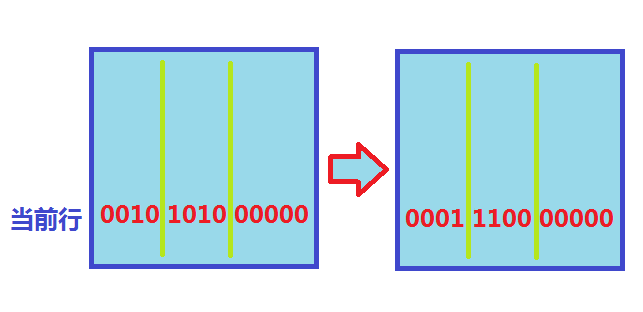
\includegraphics[width=\textwidth]{_cf243e/fig1.png}
					\caption{直接靠拢}
				\end{minipage}
				\begin{minipage}{.45\textwidth}
					\centering
					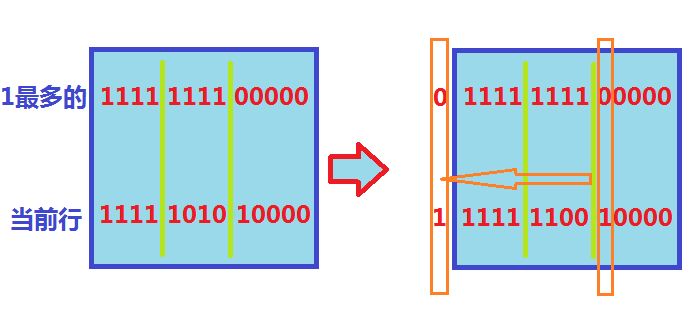
\includegraphics[width=\textwidth]{_cf243e/fig2.png}
					\caption{移动到最前面}
				\end{minipage}
			\end{figure}
		
			我们只能移动最左边和最右边有1的组,而中间的组中假设有0怎么移动也不能变得合法。所以“靠拢”完后,要检查是否使此行所有的1都靠在一起,如果不能就输出“NO”。接着我们把此行即有0又有1的组分离成两个组,一个包含0,一个包含1,我们还要确认最右侧的组是否能维持“特殊”。因为组间是有序的,这样无论以后怎么变换这行都一直会保持合法。为了使这行合法也仅此一种方案,所以如果数据有解这样一定能找到解。
		
			重复找出这样的行并执行“靠拢”,直到所有未确定是否合法的行中的1都仅在一个组中而无法执行“靠拢”。然后在这些组中再找出其中1最多的行分组,重复整个过程,直到所有的行都被标记为合法为止。
		
		\myparagraph{时空复杂度}
		
			记先找1最多的行再重复“靠拢”的过程为P,每次找行要么找到了需要“靠拢”的行,要么找不到而结束这次过程P。因为要操作的行只有n条而过程P只会递归地执行$O(n)$次,所以找行的过程一共要执行$O(n)$次。每次找行要用$O(n)$的时间扫描所有行,每次要用$O(n)$时间找出其所属组并判断是否需要操作“特殊”组,此外每次找到行后还需要使用$O(n^2)$的时间进行列的重组,所以总时间是$O(n^3)$的,空间复杂度$O(n^2)$。
	
	\section{Codeforces 249D - Donkey and Stars}
	
		\myparagraph{题目大意}
		
			天上有$n$颗星星($n \leq 10^5$),在坐标系的第一象限。假设从原点发出两条射线,相对于$x$轴的角度分别为$\alpha_1$和$\alpha_2$,可以选择这两条射线间任意一颗星星。从这颗星星作与上述射线方向相同的射线,可以再选择这两条新射线之间的星星。不断继续下去,问最多选择多少颗星星。
		
		\myparagraph{算法讨论}
		
			如果$\alpha_1=0$且$\alpha_2=90^\circ$,问题显然是要对星星求一个最长不下降子序列,即选择的星星依次$x$坐标和$y$坐标都增加。现在要对坐标系进行变换,使问题转化为最长不下降子序列。可令某星星新坐标系的横坐标$x'$为在原坐标系中到极角$\alpha_2$的射线的距离,新纵坐标$y'$为在原坐标系中到极角$\alpha_1$的射线的距离。如果记极角为$\alpha_1$和$\alpha_2$的射线对应的方向向量分别为$\boldsymbol{u}$和$\boldsymbol{v}$,则$x'=(x,y)\times \boldsymbol{v}, y'=(x,y)\times \boldsymbol{u}$。进行完坐标变化后直接做最长不下降子序列即可。
		
		\myparagraph{时空复杂度}
		
			时间只用在做最长不下降子序列上,$O(n\log_2n)$。空间$O(n)$。
	
	\section{Codeforces 249E - Endless Matrix}
	
		\myparagraph{题目大意}
		
			有一个形如下图的无穷矩阵。有$t$个询问,每次问一个子矩阵的和。如果答案超过10位,输出三个“.”,然后答案的后十位,否则输出答案。$t \leq 10^4$,询问的子矩阵范围$\leq 10^9$。
			
			\begin{figure}[ht]
				\centering
				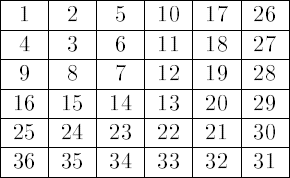
\includegraphics[width=.7\textwidth]{fig249e_1.png}
				\caption{矩阵}
			\end{figure}
		
		\myparagraph{算法讨论}
		
			首先把询问转化为求同处前$n$行和前$m$列的元素的和,记为$S(n,m)$。即如果询问的矩阵左上角为$(x1,y1)$,右下角为$(x2,y2)$,那么答案为$S(x2,y2)-S(x1-1,y2)-S(x2,y1-1)+S(x1-1,y1-1)$。
			
			现在求$S(n,m)$。记$t=\min(n,m)$,$1 \sim t^2$肯定排列在这个$n$×$m$子矩阵的左上角,先对其求和:$\frac{(t^2+1)t^2}{2}$。如果$n>m$,子矩阵的底部$n-m$行都是公差1的等差数列,第$i$行的首项$i^2$。总和为$\sum_{i=n+1}^m(i^2m+\frac{m(m+1)}{2})$,加上$\frac{(t^2+1)t^2}{2}$就是答案。如果$n<m$,子矩阵右部$m-n$列都是公差为-1的等差数列,第$i$列首项$(i-1)^2+1$。总和为$\sum_{i=m+1}^n(((i-1)^2+1)n-\frac{n(n+1)}{2})$,加上$\frac{(t^2+1)t^2}{2}$就是答案。
			
			以上式子可以用平方和公式轻松化为$O(1)$可以解决的问题。接下来要解决数值过大的问题。首先可以用实数计算判断是否要输出三个“.”,接着用整数计算精确答案。输出要对$10^{10}$取余,而$10^{10} \times 10^{10}$是会溢出任意类型的,但$10^{10} \times 10^9$恰好可以用64位无符号整形存下,而读入都是$10^9$以内的。应适当安排求值顺序,使每次乘法都不会溢出。另外等差数列求和公式中有除二,平方和公式中有除六(除二再除三)。3和$10^{10}$互质,如果要计算$x/3$,只需判断$x$、$x+10^{10}$、$x+2 \times 10^{10}$哪个可以整除3即可;但是只能在对$10^{10}$取余之前除二,观察式子,可以找到适当的地方除二的。这样依然可以在$O(1)$时间回答每个询问。
		
		\myparagraph{时空复杂度}
		
			每个询问$O(1)$。总时间$O(t)$。总空间$O(1)$。
	
	\section{Codeforces 253E - Printer}
	
		\myparagraph{题目大意}
		
			有一台打印机,每秒可以打印一张纸。有$n$个任务($n \leq 50000$),每个任务会在第$t_i$秒发给打印机,要打$s_i$张纸,有优先级$p_i$($t_i,s_i,p_i \leq 10^9$)。每秒如果有任务,打印机都会打优先级最高的任务的一张纸。现在$n$个任务中的其中一个$x$的$p_x$未知,但知道$x$中所有纸都被打完的时刻$T$,除此之外的所有$t_i,s_i,p_i$都是已知的。求这个$p_x$,以及每个任务的结束(所有纸都被打完)时间。
		
		\myparagraph{算法讨论}
		
			显然$p_x$越高$x$被打完的时间就越早,所以可以二分答案。二分答案后就是直接模拟,用一个堆储存当前正在排队的任务,每次找优先级最高的处理就好了,如果堆顶的任务打完了就将它弹出。按到达时间顺序同时扫描未处理的任务,如果此时有新的任务到达就把它加进堆。
		
		\myparagraph{时空复杂度}
		
			预处理任务:按开始时间排序$O(n\log_2n)$。二分复杂度$O(\log_2n)$。每个任务只会被加进堆一次,模拟时间$O(n\log_2n)$。总时间$O(n\log_2^2n)$。总空间$O(n)$。
	
	\section{Codeforces 254D - Rats}
	
		\myparagraph{题目大意}
		
			有一个$n$×$m$的网格($n,m \leq 1000$),每个格子要么是空的,要么是墙,要么是老鼠。你要引爆两颗手榴弹,所有与任一手榴弹距离不超过$d$($d \leq 8$)的老鼠都会被清除。这里的距离指的是连接手榴弹和老鼠的不经过墙的最短四连通路径的长度。求出一对合法的手榴弹位置,或输出无解。
		
		\myparagraph{算法讨论}
		
			$d \leq 8$是突破口。对于任意一只老鼠,肯定有一个手榴弹要在与它距离不超过$d$的地方引爆,随便选一只老鼠,做深度最深为$d$的BFS,找出所有可能位置。枚举这$O(d^2)$个位置作为其中一个手榴弹的引爆点,做深度限制为$d$的BFS找出被其清除掉的老鼠。接着,找出还活着的随便一只老鼠,这一步可以通过将老鼠储存在std::set之类的容器中快速完成。第二颗手榴弹的引爆点与这只老鼠的距离也不能超过$d$,理由同上。以这只老鼠为中心做类似的BFS,找出第二颗手榴弹可能的$O(d^2)$个引爆位置,枚举这个位置,再用一个类似的BFS检查是否所有老鼠都被清除。
		
		\myparagraph{时空复杂度}
		
			枚举第一颗手榴弹的位置耗时$O(d^2)$,每枚举一次需:(1)用$O(d^2)$时间清除一部分老鼠;(2)用$O(d^2)$枚举第二颗手榴弹的位置,每次再$O(d^2)$确认是否老鼠都被清除。共耗时$O(d^6)$,加上读入的时间$O(n^2)$,总时间复杂度$O(n^2+d^6)$。总空间复杂度$O(n^2)$。
	
	\section{Codeforces 256D - Liars and Serge}
	
		\myparagraph{题目大意}
		
			有$n$个人,有人说真话有人说谎。现在问他们每个人有多少人在说真话,他们每人给出了自己的答案$a_i$。给定$n$、$k$,问有多少种$\{a_n\}$可以判断出至少有$k$人在说谎。$1 \leq k \leq n \leq 2^8$。保证$n$是2的整数次幂。
		
		\myparagraph{算法讨论}
		
			判断出一些人在说谎当且仅当他们说出的数字和说这个数字的人的数量不相等。用DP解决。从小到大处理说每个数字的人,设$f[i][j][k]$表示当前处理到数字$i$,已经处理了$j$个人,其中有$k$人被确定是说谎者,易得转移方程:
			
			$$f[i][j][k]=\sum_{p=0}^k f[i-1][j-p][k-p] \cdot \binom{j}{p} (p\not=i) + f[i-1][j-i][k]$$
			
			这个DP是$O(n^2k^2)$的,无法通过。但是$n$为2的整数次幂,只能取9个值。可以打表通过。
		
		\myparagraph{时空复杂度}
		
			打表。打表时间$O(n^2k^2)$,实际时间$O(1)$。打表所需空间$O(n^2k)$,实际所需空间$O(n^2k)$。
	
	\section{Codeforces 264E - Roadside Trees}
	
		\myparagraph{题目大意}
		
			在一条直线有n个位置可以种树($n \leq 10^5$),自西向东标号1至n。每个月,每棵树都会长高1米。每个月初有一个操作,操作有两种类型:
			
			\begin{enumerate}
				\item 在位置p种一棵高度为h的树。($1 \leq p \leq n, 1 \leq h \leq 10$)
				\item 砍掉从西向东数的第x棵树,当这个位置的树被砍掉后,这个位置不能再种树。($1 \leq x \leq 10$)。
			\end{enumerate}
			
			每次操作后输出树高的最长上升子序列长度。
		
		\myparagraph{算法讨论}
		
			回顾用数据结构做$\{a_n\}$的最长上升子序列的方法:做到第$i$个数时,在数据结构中查询$i$之前最大的一个小于$a_i$的数是多少,用它更新最长上升子序列,插入数据结构。类似的,我们也可以扫描数列元素的值,从大到小做到值为$i$的数时,在数据结构中查询坐标大于该数坐标的最小一个坐标,用它更新最长上升子序列,插入数据结构。这两种方法本质是一样的。这里我们要结合这两种方法。
			
			同时维护上述的两个数据结构。当新种树时,一定是树高最小的10棵之一,暴力在数据结构中撤销这最小的10个,然后按上面的第二种方法重新计算,更新这种方法对应的数据结构时同时更新另一种方法的数据结构。当要砍树时,砍的树一定是最西边的10棵树之一,类似的,暴力撤销这10棵,然后重新计算。撤销时每次在数据结构中找最小(或最西)即可找到这十个,也可以另维护堆或set。
		
		\myparagraph{时空复杂度}
		
			数据结构可用线段树实现,每次种树或砍树时间复杂度$O(\log_2n)$,总时间$O(n\log_2n)$,有常数10。空间复杂度$O(n)$。
	
	\section{Codeforces 266E - More Queries to Array...}
	
		\myparagraph{题目大意}
		
			你有一个包含n个整数$a_1$,$a_2$,...,$a_n$数组。你的任务是快速地执行以下两种操作。
			
			\begin{enumerate}[leftmargin=15mm]
				\item 将闭区间{[l,r]}中的元素赋值为x。即此操作过后$a_l$,$a_{l+1}$,...,$a_r$的值都为x。
				\item 计算并输出和$\sum_{i=l}^r a_i \cdot (i-l+1)^k$,此处k不超过5。因为这个和可能很大,你要输出它模1000000007($10^9+7$)的结果。
			\end{enumerate}
			
			1≤n≤100000,初始数组中0≤$a_i$≤$10^9$。赋值操作中1≤l≤r≤n,0≤x≤$10^9$;询问操作中1≤l≤r≤n,0≤k≤5。
			
		\myparagraph{算法讨论}
		
			我们可以对0≤j≤5维护$i^j a_i$的区间和(1≤i≤n)。考虑一次询问l,r,k,例如k=2,询问的和为$\sum_{i=l}^r  a_i \cdot (i-(l-1))^2 = \sum_{i=1}^r  a_i \cdot i^2 - \sum_{i=1}^r  a_i \cdot 2i(l-1)^2 + \sum_{i=1}^r  a_i \cdot (l-1)^2$,便转换为分别询问0、1、2次$i^j a_i$的区间和。一般地,展开后用i整理可以将询问转换为0至k次的区间和,以此可以实现在知道$i^j a_i$的区间和的情况下O(k)查询。预处理$i^j$(1≤i≤n,0≤j≤5)的前缀和,即可实现插入中O(k)算出一个区间0至5次幂的区间和。以上是在假设维护了区间和的情况下,现在使用线段树维护。
			
		\myparagraph{时空复杂度}
			
			使用线段树维护区间和,时间复杂度$O(mk\log_2{n})$,空间复杂度O(n)。
	
	\section{Codeforces 267C - Berland Traffic}
	
		\myparagraph{题目大意}
		
			现有一个$n$个点$m$条边的网络。每条边有一个容量限制,对于一条边$(x,y)$,设其流量为$t$,容量为$c$,如果$t$大于0则是从$x$流向$y$,反之就是从$y$流向$x$,但$t$的绝对值不能超过$c$且可以不是整数。网络中节点1是源点,节点$n$是汇点,对于除$1,n$外的所有点,流入的流量等于流出的流量。这个网络有一个性质,对于任意一对节点$(x,y)$,$x$到$y$的路径上流量之和不会随着选择不同的路径而改变(有可能有小于0的流量,流量的符号取决于$x$到$y$路径上这条边的方向)。
			
  		求满足上述条件且流过该网络的流量尽可能大的方案以及最大的流量是多少。$n \leq 100, m \leq 5000$。
		
		\myparagraph{算法讨论}
		
			问题的关键是如何处理任意相同起点和终点的所有路径流量和都相同的限制。如果对每一个点设一个势能,令每条边的流量等于其两端点的势能差,恰好满足这个限制。这样,直接设起点势能为1,终点势能为0,其余每个点的势能为未知数,用流量平衡列出$n-2$条方程,直接解得每个点的势能。对于每个点数大于1的连通块,其中每个点的势能都有唯一解。接下来处理容量的限制:遍历每条边,求容量除以势能差,取其最小值,每条边的实际最大流量就是该边势能差乘以这个商,即取了最紧的限制。
		
		\myparagraph{时空复杂度}
		
			整个程序只需解方程和遍历每条边,总时间$O(n^3+m)$,总空间$O(n+m)$。
	
	\section{Codeforces 269E - String Theory}
	
		\myparagraph{题目大意}
			
			给一个矩形,两条竖边上分别均匀分布N个点,两条横边上分别均匀分布M个点(N,M≤$10^5$),每个点向另一个不在同一边上的点连了一条线。输出一个重排行和列的方案使这些线不相交,或输出无解。
			
		\myparagraph{算法讨论}
		
			构造出解。从一个点出发,交替地先走到与该点相连的点上,再走到与第二个点有公共行/列的点上,直到走回初始点,这样的路径称为\emph{环}。如果两条线都连接着矩形的相同两条边,那么认为这两条线的方向是相同的。如果从一个环的任意节点按任意方向出发所经的线,与从另一个环的任意节点按任意方向出发所经的线对应方向相同,则认为这两个环是相同的。注意到无论如何变换行和列的顺序,环都相同;如果两个矩形中的环都相同,其中一个矩形也一定可以通过重排行和列变换到另一个矩形。样例的环如下图用不同颜色表示:
			
			\begin{figure}[ht]
				\centering
				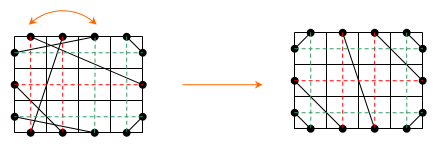
\includegraphics[width=\textwidth]{fig269e_1.jpg}
				\caption{环}
			\end{figure}
			
			有一类环只包括一条上到右的线、一条右到下的线、一条下到左的线和一条左到上的线,把这类环顺次排列到矩形的四角,设这样的环有A个。不妨考虑矩形的横边长于竖边,设有B条从上到下的线(注意不会有从左到右的线,事实上A=M-N),合法解中要么还有M-2A-B条线从上连到左、有M-2A-B条线从右连到下,要么还有M-2A-B条线从上连到右、有M-2A-B条线从左连到下(这些线不在那4A条线中),此外就没有别的线了。这2(M-2A-B)条线中,每一对有端点在同一行的,记为一组,这一组可以表示为一条从上到下的路径(注意到所有这些线都成组,每组两条线一条连接着上边,一条连接这下边),此外那B条从上到下的线也可以分别表示一条路径。这些路径的上下端点都分布在A+1$\sim$M-A列上,可以将这些列提取出来,标号为0$\sim$M-2A-1。观察到这些路径是平行的,对于上端点标号i的,下端点一定标号(i+k) mod (M-2A),k是一个整数。这样这些路径就可以写成一个列编号的轮换:
			
			$$\begin{pmatrix} 0 & 1 & ... & M-2A-1 \\ k & k+1 & ... & k-1 \end{pmatrix}$$
			
			仅由一条从上到下的线构成的路径\textbf{连续}地分布在矩形的中间,另外的由两条线构成的路径分布在两侧,所以这些路径构成了$\frac{M-2A-1}{gcd(M-2A-1,k)}$个\textbf{相同}的环,只要知道M,A,B,每个环都是已知的,依次将读入矩形中的环对应移动至这些环中即可。
		
		\myparagraph{时空复杂度}
		
			首先我们需要找出读入数据中的环,这一步是线性的。然后要找出一类环移动到矩形的四角,这一步也是线性的。对于剩下的环,用合法解的环建一个KMP,再用二倍长度的读入数据中的环匹配判断是否相同(循环同构),如果是则将其移动至对应位置,这一步也是线性的。如果以上任意一步失败则输出无解。整个过程是线性的,时间复杂度$O(N+M)$,空间复杂度$O(N+M)$。
	
	\section{Codeforces 273D - Dima and Figure}
	
		\myparagraph{题目大意}
		
			在一个$N$×$M$的网格上选择一些格子涂黑,使被涂黑的格子四连通,并且任意两个被涂黑的格子$(x1,y1)$和$(x2,y2)$间只经过被涂黑格子的最短路径长度为$|x1-x2|+|y1-y2|$。$N,M \leq 150$。求总方案数,模$10^9+7$。
		
		\myparagraph{算法讨论}
		
			题目本质是要求一个“凸”的涂黑的格子组成的连通块。假设从上到下枚举行,连通块的左端肯定是先逐渐偏向左,再逐渐偏向右;连通块的右端肯定是先逐渐偏向右,再逐渐偏向左(当然也可能只偏向左或右);并且连通块肯定是实心的。可设状态$f[i][l][r][s1][s2]$,表示当前做到第$i$行,连通块的左端在第$l$列,右端在第$r$列,s1和s2都在0/1取值,分别表示连通块的左/右端分别正在偏向左/右,$f[i][l][r][s1][s2]$表示上述限制下的方案数。总状态是$O(nm^2)$的。暴力地转移是$O(m^2)$的,但记录区间和优化即可做到$O(1)$转移。边界状态值为零,转移时每个合法状态都应+1(等同于枚举连通块上界),对所有合法的状态求和即为答案(等同于枚举连通块的下边界)。
		
		\myparagraph{时空复杂度}
		
			状态$O(nm^2)$,转移$O(1)$。故总时间$O(nm^2)$,总空间也是$O(nm^2)$。
	
	\section{Codeforces 274C - The Last Hole!}
	
		\myparagraph{题目大意}
		
			无限大的平面上有$n$个圆,圆心给定,每个圆在时刻$t$的半径都是$t$。某些时刻,平面中可能存在一些有限大的未被圆覆盖的连通块,这些连通块称为“洞”。求最早的一个时刻$x$,使时刻$x$之后都不存在“洞”,即求最晚消失的“洞”的消失时刻。$n \leq 100$。
		
		\myparagraph{算法讨论}
		
			由于数据较小,本题解法较多。我用的是下面所述的$O(n^2\log_2n)$解法。
		
			“洞”消失时,面积趋近于零,相当于一个点。这个点到包围这个“洞”的几个圆的圆心距离相同,事实上就处在所有圆心形成的Voronoi图的顶点上。也可以理解为平面上每个点都会被离它最近的圆“吞噬”,Voronoi图顶点离与它相距最近的圆最远,最后消失。由于数据较小,不必使用复杂的$O(n\log_2n)$算法求Voronoi图,可以枚举圆心$X$,确定其它圆心与圆心$X$连线的中垂线,每个中垂线将平面分为两个半平面,取包含$X$的半平面,再用这些半平面求出半平面交,就可以求出Voronoi图中与$X$连通的一块。甚至半平面交也可以用暴力算法,不过我使用的是$O(n\log_2n)$算法。这样求Voronoi图的总时间就是$O(n^2\log_2n)$。
			
			但是Voronoi图的顶点不一定都在“洞”里,一个Voronoi图的顶点要在“洞”里,必须被若干个圆包围。Voronoi图的顶点的个数是线性的,枚举Voronoi图的顶点,扫描与这个顶点相邻的圆心,对它们按与这个顶点的相对极角排序,扫描每个与其相邻的圆心,判断每个圆心与上一个圆心的极角之差是否都在$180^\circ$以内。如果都在,那么这个Voronoi顶点就在“洞”里。这一步要扫描$O(n)$个顶点,并对$O(n)$个圆心进行排序并扫描,时间也是$O(n^2\log_2n)$。
			
			对于每个在“洞”里的Voronoi顶点,计算它和与它相邻的圆心的距离,这个距离就是这个“洞”消失的时间。答案就是这个距离的最大值。
		
		\myparagraph{时空复杂度}
		
			两步的时间都是$O(n^2\log_2n)$,总时间$O(n^2\log_2n)$。总空间$O(n)$。
	
	\section{Codeforces 274E - Mirror Room}
		
		\myparagraph{题目大意}
			
			给一个n×m的网格,有k个格子是镜子(1≤n,m≤$10^5$,0≤k≤$10^5$)。光从一点发出,遇到镜子会像下图一样反射:
			
			\begin{figure}[ht]
				\centering
				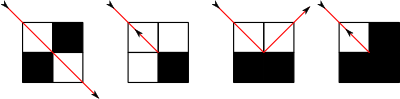
\includegraphics[width=\textwidth]{fig274e_1.png}
				\caption{反射}
			\end{figure}
			
			求光路会经过多少个格子,重复经过不计。
			
		\myparagraph{算法讨论}
		
			一个可行的方案是直接用复杂的数据结构模拟,直到光路进入循环,但是题目中的一些性质可以使解法更简单。首先显然光会以原方向回到起点才进入循环,其次光不会以交叉的方向通过同一个格子两次,这点对格子黑白染色后就能发现,这样就省去了判重的步骤。先处理出每个反射点,对每条对角线都建一个数据结构(C++可用set,也可以不建数据结构而使用二分),插入反射点。直接进行模拟,每次可在数据结构上找出光的下一个反射点的位置以及反射后的方向,对光路上的每条线段累加其长度即可,直到回到起点。对于中途“掉头”的光路,可分起点前和起点后两部分分别计算。
		
		\myparagraph{时空复杂度}
		
			我们是统计不重复的光路,光路上的反射点最多$O(n+m+k)$个,数据结构的时间$O(\log_2k)$。总时间复杂度$O((n+m+k)\log_2k)$,空间复杂度$O(n+m+k)$。
	
	\section{Codeforces 280E - Sequence Transformation}
	
		\myparagraph{题目大意}
		
			给一个不递减序列$\{x_i\},(1 \leq i \leq n, 1 \leq x_i \leq q)$,要求把序列转化为新序列$\{y_i\},(1 \leq i \leq n, 1 \leq x_i \leq q)$,并满足$a \leq y_{i+1}-y_i \leq b,(1 \leq i < n)$,转化代价为$\sum_{i=1}^n(y_i-x_i)^2$。找出使代价最小的$\{y_i\}$。($1 \leq a,b,q \leq 10^9, 1 \leq n \leq 300000$,数据比CF原题的大)
		
		\myparagraph{算法讨论}
			
			记$y_i=v$时的代价函数为$f_i(v)$,假设$f_i$是一个先递减后递增的函数,记其最小值点为$v=min$,设
			
			$$\begin{aligned}
				g_i(v)&=\min_{v-B \leq v' \leq v-A}f_i(v')\\
				      &=\begin{cases}
				           f_i(v-A) & v < min+A \\
						   f_i(min) & min+A \leq v < min+B \\
						   f_i(v-B) & v \leq min+B
						\end{cases} \\
				f_{i+1}(v)&=\min_{v-B \leq v' \leq v-A}f_i(v')+(v-x_{i+1})^2 \\
				          &=g_i(v)+(v-x_{i+1})^2
			\end{aligned}$$
			
			显然$f_1(v)=(v-x_1)^2$是一条开口向上的抛物线,是先递减后递增的函数。$f_i$每次变换为$g_i$后显然还是先递减后递增的函数,再加上$(v-x_{i+1})^2$后,因为两个导数递增的函数相加依然导数递增,$f_{i+1}$依然保持此性质,故上述转移可行。
			
			每次转移我们需要的操作是 1.查找一个先递减后递增函数的最小值 2. 将函数的一部分左右平移。 3. 在函数中插入一段。 4. 将函数整体加上一个二次函数。 因为$f_i$的每一段都是一个二次函数的一部分,可用一个平衡树维护其每一段,并执行上述操作,以此做到快速转移。最后查找$f_n$的最小值即最优解。记录下每一次转移的$min$值,即可由最后的最小值逆推回每个$y_i$。
			
		\myparagraph{时空复杂度}
		
			$O(n)$次转移,每次耗时$O(\log_2n)$,总时间复杂度$O(n\log_2n)$。每次转移在函数中最多新增一段,空间复杂度$O(n)$。
	
	\section{Codeforces 286D - Tourist}
	
		\myparagraph{题目大意}
		
			有些时刻会有点$A(1,0)$和$B(-1,0)$同时以1单位每秒的速度向$y$轴正方向移动,而另某些时刻会有墙出现,从$(0,l)$延伸到$(0,r)$。墙瞬间出现,且出现后就不消失,而且多堵墙间可以有重叠。问对于每对$(A,B)$,在其运动过程中有多少秒$AB$连线会与至少一堵墙相交。共$n$对$(A,B)$、$m$堵墙,$n,m \leq 10^5$。
		
		\myparagraph{算法讨论}
		
			建立另一个坐标系$y-t$,$A$和$B$的轨迹在其上对应一条斜率为1的射线,表示在每时刻它们的$y$坐标为多少。对每堵墙作矩形:记其出现时刻为$t$,它的左下角为$(t,l)$,左上角为$(t,r)$,向右无限延伸。这样问题可以转化为$A$和$B$对应的射线与任意矩形相交部分的总长为多少(答案要乘$\frac{\sqrt{2}}{2}$)。
			
			由于墙可能有重叠,要先把它处理成不重叠的以便后续工作。把墙对应的矩形按左边界的$t$坐标从小到大排序,用一个std::set或其他类似数据结构记录其上下边界的$y$坐标。每添加一个新的矩形,查找它与哪些已添加的矩形相交。如果与新添加矩形相交的矩形的$y$坐标区间被新矩形的$y$坐标区间完全包含了,就结束被包含的矩形,即将其右边界设为新矩形的左边界。如果只被部分包含,就缩小新矩形的范围使之不再相交。
			
			现在,为了方便,将坐标系作如下变换:$(t,y) \to (t-y,y)$。这样$(A,B)$对应的射线就平行于$y$轴了,而且答案不再需要乘$\frac{\sqrt{2}}{2}$了。此时原来的矩形变成了梯形,其左边的斜率为-1。再次为了方便,可以将其看成一正一负两个三角形。记该三角形的最左边的顶点坐标为$(p,q)$,若它与$(A,B)$对应的射线(记其为$t=t0$)相交,那么它对答案的贡献为$t-p$,即总答案为:$t$乘以与射线相交的三角形个数,减去与射线相交的三角形的$p$之和。将三角形和射线都按按新坐标系的$t$坐标从小到大排序,从小到大扫描并维护答案即可。
		
		\myparagraph{时空复杂度}
		
			去除墙的重叠需使用set,时间$O(m\log_2m)$。最后的扫描需将墙和射线都排序,时间$O(m\log_2m + n\log_2n)$。总时间复杂度$O(m\log_2m + n\log_2n)$。总空间复杂度$O(n+m)$。
	
	\section{Codeforces 286E - Ladies' Shop}
	
		\myparagraph{题目大意}
		
			有$n$个包($n \leq 10^6$)用来装物品,每个包有大小$p_i$,现在要确定物品的大小的种类(每个大小有无限个物品)满足这样的要求:
			
			\begin{enumerate}
				\item 对于每个包都可以找到一些物品恰好塞满这个包。
				\item 从这些物品中选出任意一些总大小不超过$m$的($m \leq 10^6$)都有一个包可以正好用它们装满。
				\item 使物品大小的种类数尽量小。
			\end{enumerate}
		
		\myparagraph{算法讨论}
		
			为了满足条件2,选出的物品大小必须是原来包的大小的子集。也因为条件2,任意两个包的大小之和($m$以内)必须是另一个包的大小(①)。如果一个包的大小等于两个比它小的包的大小之和,那么就不需要再有和这个包一样大的物品了,反之需要(②)。可以把问题转化为卷积:设$m$次界多项式$P$,对于所有$p_i$次项的系数为1,否则为0。检验$P^2$的系数,如果不是包大小的系数非零,则无解(①);如果是包的大小的系数为零,那么这个大小就是一个物品的大小(②)。使用FFT实现。
		
		\myparagraph{时空复杂度}
		
			FFT。时间复杂度$O(m\log_2m)$,空间复杂度$O(m)$。
	
	\section{Codeforces 294D - Shaass and Painter Robot}
	
		\myparagraph{题目大意}
		
			给你一个$n \times m$的网格,一开始都是白色的。上面有一个机器人,一开始位于格子$(x_s,y_s)$上(占据整个格子),面朝某个方向(左上,左下,右上,右下之一)。然后机器人会一直顺着这个方向走下去,每当遇到边界时会遵循光的反射定律改变方向,然后继续走。每当机器人走到一个格子后,它会将这个格子染黑,用掉一个单位颜料。即便这个格子已经被染黑了,也需要耗费一个单位颜料。当机器人意识到这个$n \times m$的网格已经变成黑白相间的时候,它会立即停止行动。现在希望你求出,机器人停下来的时候,已经耗费了多少颜料?或者指出永远不可能停下来。$n,m \leq 10^5$。
			
		\myparagraph{算法讨论}
		
			如果机器人只有在需要转弯的时候才判断是否停止,染色完成的充要条件是所有边界上的应该染色的格子都被染了。
			
			\begin{proof}必要性显然。如果有一个不在边界上的格子$A$没有被染色,那么与它同处一条对角线上(不一定是主对角线)的边界上的四个格子也不可能被染色,因为边界上的格子只有最多两个方向可以出入,要到达边界上的格子必须同时染色这两个方向上的格子,而$A$就在其中一个方向上。就算边界上的其中一个格子是起点,也有剩下三个格子决定了$A$一定会被染色。\end{proof}
			
			很容易可以推出,机器人停止时要么是准备转弯时,要么是以与出发相同的方向回到原点时。如果不是第一种情况,机器人肯定不是在边界上出发的,可以先让机器人移动到边界上再计数,这样可以只在每次需要转弯时判断是否停止而不影响答案。
			
			接下来,就可以直接模拟机器人的动作,模拟时记录已经走过了哪些边界上的格子。显然,机器人如果还没完成染色就走到了以前走过的格子上,那它一定永远停不下来。边界上只有$O(n+m)$个不同格子,最多只需模拟$O(n+m)$次行走,每次算出走到下一个需要转弯的格子需要花多少步,再判断是否已经染色完成即可。
			
		\myparagraph{时空复杂度}
		
			$O(n+m)$次模拟,每次$O(1)$计算,总时间$O(n+m)$。用总空间$O(n+m)$记录已经走过哪些边界上的格子。
	
	\section{Codeforces 297E - Mystic Carvings}
	
		\myparagraph{题目大意}
		
			有一个圆上分布着$2n$个点($n \leq 10^5$),这些点组成给定的$n$对,每个点在且仅在一对中。现在要找出3对点,使属于同一对的两个点的距离相等。此处距离定义为这两个点间属于这6个点的点的个数+1。输出取这3对点的方案数。
		
		\myparagraph{算法讨论}
		
			不管合不合法,选出这3对点只有如图5种情况。
			
			\begin{figure}[ht]
				\centering
				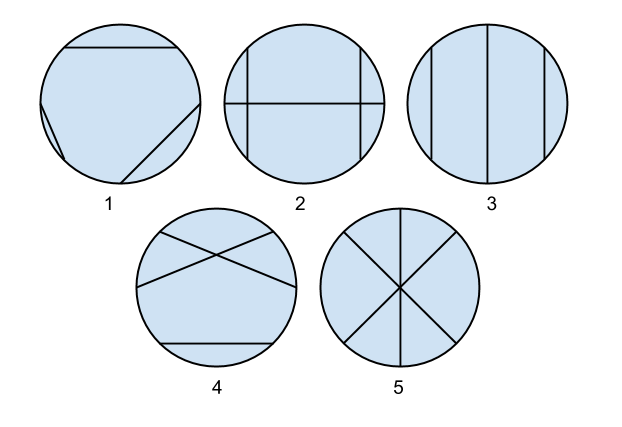
\includegraphics[width=0.8\textwidth]{fig297e_1.png}
				\caption{选出3对点(连线表示一对)}
			\end{figure}
			
			只有第1种和第5种合法。第5种的方案比较难算,第1种也不简单,可以考虑用总数减去不合法的方案数。假设在每一对的两个点间连线,假设我们可以算出与任意一条线$i$相交、在其一侧、在其另一侧的线的数目,分别记作$x_i$、$y_i$、$z_i$。第2种情况和第4种情况都是有两条这样的线,有另外一条线与它相交,一条与它不相交,所以这两种情况的总数为$\frac{1}{2}\sum_i x_i(y_i+z_i)$。第3种情况则是有一条这样的线,它两侧各有一条线,这种情况的总数为$\sum_i y_i z_i$。所以答案为
			
			$$ \binom{n}{3}-\frac{1}{2}\sum_i x_i(y_i+z_i)-\sum_i y_i z_i $$
			
			现在问题只剩怎么求$x_i$、$y_i$、$z_i$。在圆周上建一个树状数组。顺次扫描圆周,每遇一个点,假设与它成对的点还没遇到过,就把这个与它成对的点加入树状数组。在适当的时候查询树状数组即可得到一对点中一个在某区间,另一个在另外某区间的点对的数目。比如用在扫描到$r$时查询到的$(l,r)$区间中的点的数目,减去扫描到$l$时查询到的$(l,r)$区间中的点的数目,可得两点都在$(l,r)$中的点对的数目。这样既可求得$x_i$、$y_i$、$z_i$。
		
		\myparagraph{时空复杂度}
		
			扫描圆周,每次在树状数组上插入和询问,总时间复杂度$O(n\log_2n)$。总空间复杂度$O(n)$。
	
	\section{Codeforces 303D - Rotatable Number}
	
		\myparagraph{题目大意}
		
			如果一个长度为$n$的数乘1、乘2、……、乘$n$,可以得到所有由它旋转得来的数,则称此数为可旋转数,旋转指将此数的前若干位移至最后。如$142857 \times 2=285714$,285714相当于把14移至末尾。给定$n$,求最大的$1<b<x$,使$b$进制下存在长度为$n$的可旋转数。$1 \leq n \leq 5 \times 10^6, 2 \leq x \leq 10^9$。
		
		\myparagraph{算法讨论}
		
			每个长度为$n$的可旋转数对应一个分数$\frac{1}{n+1}$。记$p=n+1$,这个分数为$\frac{1}{p}$,这个分数对应循环节为$n$的循环小数,如$\frac{1}{7}=0.\dot{1}4285\dot{7}$。此例中,$\frac{2}{7}=0.285714, \frac{3}{7}=0.428571, \cdots$,分别相当于旋转。$0.\dot{1}4285\dot{7}=\frac{142857}{999999}$,反过来,就可以将这个可旋转数表示为
			
			$$\frac{b^{p-1}-1}{p}$$
			
			但直接这样构造不一定合法。首先这个数要是循环小数,这要求$p \nmid b$。其次,这个循环小数的每一位均不相同,这样$\frac{1}{p}, \frac{2}{p}, \cdots, \frac{n}{p}$就对应不同的循环小数。这个循环小数的每一位分别等于$b^0 \mod p, b^1 \mod p, \cdots, b^n \mod p$,显然每一个循环小数之间都会是循环同构的。为了使每一位不等,$p$应为质数且$b$应是模$p$意义下的原根。
			
			这样问题就转化为找出最大的一个$b$使$p \nmid b$且$b$是模$p$意义下的原根。可以从大到小枚举$b$,每次判断$b^{\frac{p-1}{2}}, b^{\frac{p-1}{3}}$等模$p$是否为1即可。
		
		\myparagraph{时空复杂度}
		
			因为是在模$p$同余系下枚举$b$,可能的值不超过$p$个,时间$O(n)$。每次要判断$\sqrt{p}$个数是否为1,还要用$O(\log_2n)$的时间执行快速幂。总时间$O(n^{1.5} \log_2n)$。空间$O(1)$。
	
	\section{Codeforces 303E - Random Ranking}
	
		\myparagraph{题目大意}
		
			有$n$个学生($n \leq 80$)进行一次考试,每个学生$i$的成绩在实数区间$[l_i,r_i]$间均匀随机分布。对于所有$i$、$j$,问学生$i$排名第$j$的概率。
		
		\myparagraph{算法讨论}
		
			将成绩离散化,分成总共最多$2n$个区间。逐一确定每个学生的排名的概率。枚举学生$i$,再枚举他的成绩分布在区间$j$中。因为他的排名只决定于剩下的学生中有多少个成绩在他前面,所以可逐个计算剩下的学生。设状态$f[p][q][r]$表示目前计算了剩下$n-1$个学生中的$p$个,有$q$个的成绩落在区间$j$之前,有$r$个恰好落在了区间$j$。转移时只需分别计算学生$p$的成绩落在区间$j$之前、之后和恰好落在$j$上的概率即可,转移是$O(1)$的。显然,$f[p][q][r]$对$i$排名在$q+1 \sim q+r+1$都有贡献$f[p][q][r]/(r+1)$。这样整个算法是$O(n^5)$的。
			
			上面的时间复杂度看起来是不能过的,可以尝试优化。注意到$j$相同时,对于每个$i$都要计算除了$i$外的所有人,其中有许多重复。我们可以先枚举$j$,然后进行分治。上述DP中枚举$p$的顺序是无关紧要的,假设$i$在区间$[l,r]$中,我们已经计算好了区间$[l,r]$外的所有$p$,记$mid=(l+r)/2$,假设$i$在$[l,mid]$中,我们就在$[mid+1,r]$中枚举$p$进行转移,递归进区间$[l,mid]$继续计算,否则$i$在$[mid+1,r]$中,我们就在$[l,mid]$中枚举$p$进行转移,同样递归下去。只要记录$f$数组的中间结果,就可以将枚举$i$和$p$的总时间降到$O(n\log_2n)$,算法总时间$O(n^4\log_2n)$。
		
		\myparagraph{时空复杂度}
		
			上面的第二种算法时间复杂度$O(n^4\log_2n)$,空间复杂度$O(n^3)$。看起来第二种算法更优,但是由于①$n$较小,②而且第二种算法要先枚举$j$,因而不能在已知$i$的情况下用$l_i$和$r_i$确定$j$的枚举范围,③又因为第二种算法的转移需要在$O(n^3)$规模的数组上进行而第一种算法可以压维,第二种算法相比第一种算法并不占优势,反而可能更慢,甚至有过不了的风险。在本题的条件下,采取第一种算法或许是更好的选择。
	
	\section{Codeforces 306C - White, Black and White Again}
	
		\myparagraph{题目大意}
			
			会发生$w$件两两不同的好事和$b$件两两不同坏事,每天至少发生一件事,每天要么全部发生好事要么全部发生坏事。这n天会先有若干天发生好事,再有若干天发生坏事,再有若干天发生好事。(若干指大于零)要求统计事件发生的方案数(每天发生的事的顺序也不一样),答案取模$10^9+9$输出。$n,w,b \leq 4000$。
			
		\myparagraph{算法讨论}
		
			$w$件好事共$w!$种排列,$b$件坏事共$b!$种排列,互不影响。要将坏事插入到好事种,有$w-1$个间隙,即$w-1$种方法。最后要将这些事分成$n$天,好事和坏事间的界限已经分好了,还需要在$w+b-3$个可能位置中插入$n-3$个间隔,有$\binom{w+b-3}{n-3}$种。
			
			答案为$w!b!(w-1)\binom{w+b-3}{n-3}$。乘法直接计算。除法用快速幂求逆元计算。
		
		\myparagraph{时空复杂度}
		
			计算阶乘$O(max(n,w,b))$,计算快速幂用对数时间。总时间可认为是$O(max(n,w,b))$,总空间$O(1)$。
	
	\section{Codeforces 306D - Polygon}
	
		\myparagraph{题目大意}
		
			对于给定$n$($3 \leq n \leq 100$),构造任意一个合法多边形,满足其所有内角相等,任意两个边长的差的绝对值大于等于$10^{-3}$,边长$\in [1,1000]$,横纵坐标的绝对值小于等于$10^6$。
		
		\myparagraph{算法讨论}
		
			首先,直观地看,$n$越大角度相同的限制的影响越小,可以发现$n \leq 4$时是无解的,其它情况都有解。一个很自然的想法就是对多边形的每条边按一个方向(比如逆时针)逐一随机其长度,每条边相对于上一条边旋转一个角度。但这样可能构不成多边形,原因有两种:末边未能与多边形接合、末边不是与起点而是多边形的其它部分接合了。如图:
			
			\begin{figure}[ht]
				\centering
				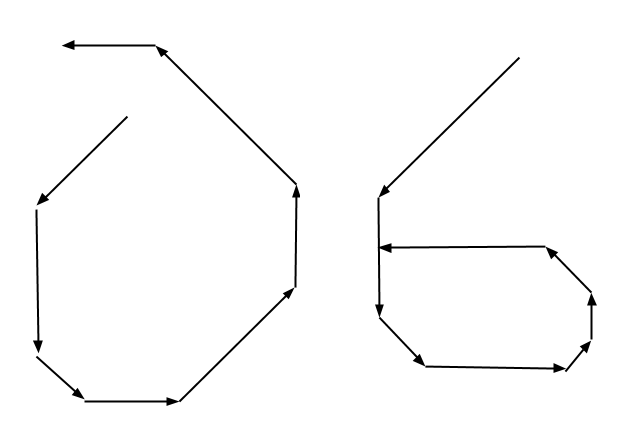
\includegraphics[width=0.6\textwidth]{fig306d_1.png}
				\caption{n=8时两种不能构成多边形的情况}
			\end{figure}
			
			首先对其进行粗略的修正。对于第一种情况,只需限制任何边不得超过初始边所在直线即可。对于第二种情况,对于任意边A,过多边形起点作A的下一条边的平行线,显然A至少要穿过这条平行线才有解。如图:
			
			\begin{figure}[ht]
				\centering
				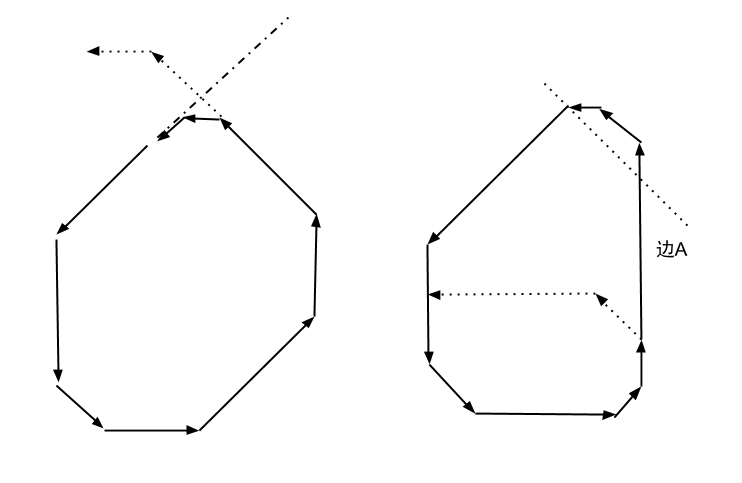
\includegraphics[width=0.6\textwidth]{fig306d_2.png}
				\caption{n=8时两种不能构成多边形的情况}
			\end{figure}
			
			显然这两种限制都只是得出合法解的必要条件,还有一个重要因素是题目中边长的限制。如果仅要求边长大于等于0而不是大于等于1,并且没有边长不相等的限制,则可以看出仅按上述限制是可以构造出解的。在有了边长限制后,就不能使某一条边只是恰好达到了上述限制,还要为后续的边长限制预留空间。需要预留的空间与剩余边数有关,剩余边数越大需要预留的空间越大。这一点比较难计算,但因为读入总共只有98种情况,又可以很轻松地写出检验程序,我们可以调整参数多次尝试。当然,也不能只是把预留空间尽量留大,因为要考虑到边长还有上限1000,而且随机的范围不能太小,以免有两边的长度过于接近。综合以上因素调整参数即可。
		
		\myparagraph{时空复杂度}
		
			实现上,只需依次在一定范围内随机每个边长,每次计算是$O(1)$的,总时间$O(n)$。总空间$O(1)$。
	
	\section{Codeforces 309D - Tennis Rackets}
	
		\myparagraph{题目大意}
		
			有一个等边三角形,每边上有$n$个$n+1$等分点。要在每边上分别选一个点,而且每条边都不能选靠近三角形顶点的$2m$个点,使选出的三个点形成钝角三角形。求方案数。$n \leq 32000$。
		
		\myparagraph{算法讨论}
		
			显然,若已知选出的其中两个点,不管在新三角形中是一个钝角顶点一个锐角顶点,还是两个锐角顶点,都是可以在$O(1)$时间内算出另一个点的,这样可以构造$O(n^2)$算法。不过,这就是时间复杂度最快的方法,所以要进行常数优化。
			
			由于时间复杂度很大,达到了$32000^2$,直接实现的常数也不大,影响常数优化的每个细节都要考虑。并且,有时常数优化不是语句和表达式看起来简短就能使程序快的,要多在自己的机子上尝试,然后找出最快的写法。当然运气好也可以一下子通过,应根据具体语句分析。下面给出若干个需要考虑,但不一定要完全遵循的地方:
			
			\begin{enumerate}
				\item 利用对称性将时间折半。如果枚举的是两个锐角顶点,这两个点离钝角顶点所在边的距离分别为$a$和$b$与分别为$b$和$a$的方案数是相同的。如果枚举的是一个钝角顶点和一个锐角顶点,那么钝角定点距离其所在边一段$a$和$N+1-a$时的方案数是相同的。
				\item 是解方程还是利用单调性维护?枚举出两点$A$和$B$后,$C$的范围可以解方程得出,虽然语句短,但这样需要开平方或者除法。事实上$C$的范围是单调的,可以直接维护一个变量表示,判断时只需乘法和加法,反而更快。
				\item break。因为上述$C$的范围是单调的,制定适当的循环顺序,当$C$范围为空时可break。
				\item 预处理循环范围。与上面相似,可以解方程直接得出循环范围,这样不仅能像break一样提早结束循环,还能推迟循环开始。不过经测试这样提升的速度并不能超过随机误差。
				\item 是枚举两个锐角点还是一个钝角点一个锐角点?经实验后者所需循环次数更少。
				\item 避免复杂的表达式而用变量维护?$C$的范围表达式比较复杂,可以考虑用一个变量维护,每次加上此次与上一次的差。这对时间的贡献应具体情况具体分析。
				\item 一些其他的因素。有时看似更慢的表达式更快,应多次尝试。此外,我发现诸如变量是开局部变量还是全局变量等因素对事件都是有影响的。
				
			\end{enumerate}
		
		\myparagraph{时空复杂度}
		
			时间复杂度$O(n^2)$,空间复杂度$O(1)$。
	
	\section{Codeforces 311C - Fetch the Treasure}
	
		\myparagraph{题目大意}
		
			有$h$间房间,从左到右编号$1 \sim h$。有$n$间有宝藏,第$a_i$间有$c_i$宝藏。可以从第一间出发探险,每次可以向右走$k$步,不可以回头。现在有$m$组操作,每组可以是
			
			\begin{enumerate}
				\item 增加走法。增加走法$x$,每次探险时还可以选择向右走$x$步而不是$k$步。增加的走法可以累积,即以后还能再增加其它的走法而这种走法仍然保留。$x \leq h$。
				\item 读入$x,y$,$a_x$减少$y$。
				\item 执行一次探险,询问路上能遇到的有最多宝藏的房间有多少宝藏,并将其取走,即此$c_i$此后为零。
			\end{enumerate}
			
			$h \leq 10^{18}, n,m \leq 10^5, k \leq 10^4, \mbox{第一种操作次数} \leq 20$
		
		\myparagraph{算法讨论}
		
			注意$k$很小。假设某次探险到达了房间$x$,那么也可以到达$x+pk$,($p$为整数)。可以将所有房间按模$k$的值整理成若干组,假设最左在房间$x$进入了某组,那么此组内编号大于$x$的房间都能到达。对每组房间建一个节点,用操作1增加的转移作为边,用最短路即可求出每组最左可在哪个房间到达。每次做操作1时做一次最短路即可。
			
			由于走法只会增加不会减少,每组最左能到达的节点只会越来越左。对每组维护一个数组,从大到小包含此组内所有有宝藏的房间。再维护一个堆,用堆维护能访问到的房间中宝藏最多是哪间,每次最短路更新后直接从这些数组更新堆即可,数组中每个元素只会从数组进入堆一次。对于操作2,也可以直接使用懒惰删除实现。
		
		\myparagraph{时空复杂度}
		
			每次操作1后要做最短路,点数为$k$,若用狄杰斯特拉,耗时$O(\mbox{第一种操作次数}k\log_2k)$。用堆维护最大值的过程中,每个有宝藏的房间都会进入堆,用操作2更新宝藏数目时也会操作堆,耗时$O((n+m)\log_2(n+m))$。总时间$O(\mbox{第一种操作次数}k\log_2k+(n+m)\log_2(n+m))$。总空间$O(n+m+k)$。
	
	\section{Codeforces 311E - Biologist}
	
		\myparagraph{题目大意}
		
			有$n$只狗,不是雄就是雌。给狗$i$做变性手术要$v_i$价钱。有$m$个富人,第$i$个富人希望$d_{i,1} \sim d_{i,k_i}$这些狗(编号不一定连续)为性别$s_i$,如果他满足了,你就可以赚$w_i$的钱。另外如果他是你朋友,他没满足,你就要亏$g$的钱。问最大收益或最小亏损。$n \leq 10^4, m \leq 2000, k_i \leq 10$。
		
		\myparagraph{算法讨论}
		
			用最小割解决。对每只狗$x$建两个点$male(x)$和$female(x)$,对每个富人$y$建一个点$folk(y)$,记一个特别大的数为$big$,记原点为$S$,汇点为$T$。
			
			对于每个$x$,连接$S$到$male(x)$,容量为$big$,如果这条狗是雌的就再加$v_i$容量,割去此边表示这条狗应为雄性;连接$female(x)$到$T$,容量为$big$,如果这条狗是雄的就再加$v_i$容量,割去此边表示这条狗应为雌性;连接$male(x)$到$female(x)$,容量为无穷大。显然不可能既不选择这条狗为雄性也不选择这条狗为雌性,而且因为有$big$,这条狗也不能同时为雄性和雌性。
			
			对于每个$y$,如果$s_i$为雄,连接所有$male(d_{y,i})$到$folk(y)$,容量无穷大;再连接$folk(y)$到$T$,容量为$w_y$,如果是朋友容量就加上$g$。如果$s_i$为雌,连接$folk(y)$到所有$female(d_{y,i})$,容量无穷大;再连接$S$到$folk(y)$,容量为$w_y$,如果是朋友容量就再加上$g$。显然只要有一条狗的要求未满足,连接$folk(y)$与源或汇的边就要被割,割的大小相当于相对于赚了$w_i$亏了多少。
			
			执行最大流算法,答案为$n \cdot big + \sum_i w_i - \mbox{流量}$。
		
		\myparagraph{时空复杂度}
		
			共$O(n+m)$个点,$O(n+\sum_i k_i)$条边。用Dinic算法时间$O(V^2E)$,即时间$O((n+m)^2(n+\sum_i k_i))$。空间$O(n+m+\sum_i k_i)$。
	
	\section{Codeforces 314E - Sereja and Squares}
	
		\myparagraph{题目大意}
		
			有一个长度为$n$的字符串($n \leq 100000$),包含大写字母和小写字母,但不包含‘x’和‘X’。这个串需要满足如下性质:串上的字符可被分成若干对,每个字符都恰好属于一对,并且每对包含一个小写字母和一个相对应的大写字母,小写字母在左侧,大写字母在右侧。还要满足对与对之间互不相交(即不存在对A和对B,B中一个字符在A两字符之间,而另一个不在)。现在这个串有些位置的字符是确定的,这些确定的位置都是小写字母,有些位置是任意的,求构成合法串的方案数,对4294967296取模。
			
		\myparagraph{算法讨论}
		
			这个串本质上是一个括号序列,小写字母就是左括号,大写字母就是右括号,对应的左右括号必须是对应的大小写字母。可设状态$f[i][j]$表示现在处理完了前$i$个字符,括号有$j$层,显然有
			
			$$f[i][j]=\left\{\begin{aligned}
				&f[i-1][j-1], &(\mbox{第$i$位是确定的,此时只能选择一种左括号})\\
				&f[i-1][j-1]*25+f[i-1][j+1], &(\mbox{第$i$位是任意的,此时可以选择25种左括号,}\\
				&							 &\mbox{但右括号只能选择与前面左括号成对的一种})
			\end{aligned}\right.$$
			
			这样的DP是$O(n^2)$的,看起来一定不能过。但只需要做一些常数优化就可以让它变得很快。
			
			首先,第一种转移相当于DP数组整体右移一位,第二种转移相当于数组整体左移一位,再做$f[i]+=f[i-2]*25$。数组整体移动时就没必要整体赋值了,直接移动标记数组左右边界的两个指针即可。这样做的另一个好处就是,数组只用开一维的大小。
			
			第二,$j$的最大值肯定不会超过已有的左括号数上限$i$,也不会超过将会有的右括号数上限$n-i+1$,依此可以限制$j$的循环范围。
			
			第三,答案对$4294967296=2^{32}$取模,可以用32位无符号整数储存值,让它自然溢出。
			
			最后把一些语句细节实现好,尽量减少循环内的比较、赋值、运算次数,就可以通过了。
		
		\myparagraph{时空复杂度}
		
			时间复杂度看起来仍然很大,是$O(n^2)$,空间复杂度$O(n)$。
	
	\section{Codeforces 316D3 - PE Lesson}
	
		\myparagraph{题目大意}
		
			有$n$个人,每个人手里有一个球,每次可以交换两个人手里的球。每个人都最多只能交换两次,而且其中有些人最多只能交换一次。求最后形成的球的排列的总数。$n \leq 1000000$。答案对$10^9+7$取模。
		
		\myparagraph{算法讨论}
		
			将整个过程看作一次置换,它可以被唯一分解为若干不相交轮换的合成。假设有轮换$(x_1,x_2,\cdots,x_n)$,它可以被看成相继进行轮换$(x_{n-1},x_n),(x_{n-2},x_{n-1}),\cdots,(x_1,x_2)$。除了$x_1$和$x_n$被交换了一次以外其它的都被交换了两次。因此每个轮换至多含两个最多交换一次的人。
			
			设有$n$个最多交换一次的人和$m$个最多交换两次的人。先只考虑那$n$个人,设这个方案数为$f_n$,那么$f_n=f_{n-1}+(n-1)f_{n-2}$,即依次考虑每个人,$f_{n-1}$表示这个人单独形成一个轮换,$(n-1)f_{n-2}$表示这个人与别人形成一个轮换,那个另外的人以后就不能形成新的轮换了。
			
			再考虑那$m$个人。依次考虑每个人,这些人可以插入到已有的轮换中(当前有多少个人就有多少插入方法),也可以新组成一个长度为1的轮换(一种方法)。所以答案要在只考虑$n$个人的基础上乘上$\prod_{i=n}^{n+m-1}(i+1)=\frac{(n+m)!}{n!}$。总方案数
			
			$$\frac{(n+m)!}{n!}f_n$$
			
			直接计算即可。
		
		\myparagraph{时空复杂度}
		
			直接计算上述公式,时间$O(n)$,空间$O(1)$。
	
	\section{Codeforces 316G3 - Good Substrings}
		
		\myparagraph{题目大意}
		
			给定一个字符串$s$和$n$个三元组$(p_i,l_i,r_i)$,要求算出满足如下要求的$s$的不同子串的个数(相同子串不计):该子串在每个$p_i$中出现次数在区间$[l_i,r_i]$中。字符串$s$和$p_i$的长度均不超过50000,$0 \leq n \leq 10$。
		
		\myparagraph{算法讨论}
		
			把所有读入的$n+1$个字符串串联起来,中间用未出现过的不同字符隔开,建一个后缀数组。对于$s$的每个后缀$t$,考虑这个后缀有多少个前缀满足要求。假设满足要求的前缀长度为$l$,有多少个来自$p_i$的后缀与$t$的LCP不小于$l$,该前缀就在$p_i$中出现了多少次。因为后缀数组中与$t$的LCP在$rank[t]$两侧是单调的,所以满足要求的$p_i$的后缀都在一个范围内连续分布,所以可以根据$l$二分出此范围。对于每个$i$预处理出一个前缀和,其中的第$j$个元素表示在后缀数组中前$j$个后缀中出现了多少次来自$p_i$的后缀,这样就可以根据上述范围判断$l$是否大了或小了。据此可以二分出$l$的区间。对于每个$t$累加$l$的区间长度即为答案。
		
		\myparagraph{时空复杂度}
		
			记读入的字符串总长为$L$。首先建立后缀数组,使用倍增法的时间为$O(L\log_2L)$。为了在$O(1)$时间内求LCP,还要用$O(L\log_2L)$的时间预处理$height$数组的RMQ。求解时,先二分$l$。对于每个$l$,先$O(\log_2L)$二分出满足要求的后缀范围,再利用前缀和$O(n)$判断是否合法。综上,总时间复杂度为$O(L\log_2L+\log_2L(\log_2L+n))$。总空间复杂度$O(L\log_2L)$(RMQ)。
	
	\section{Codeforces 317C - Balance}
	
		\myparagraph{题目大意}
		
			有$n$个容器,每个容量$v$,其间连了$e$条无向管道,管道容量无限制。每个容器初始有$a_i$水,需要在最后达到$b_i$水。每次可以选择有管道连接的两个容器,从其中一个流若干水到另一个。不同的管道中不能同时有水流动,任意时刻容器也不能溢出。要求构造一个合法的流动方案,总流动次数不应超过$2n^2$。$n \leq 300, e \leq 50000, v \leq 10^9$。
		
		\myparagraph{算法讨论}
		
			一个连通块中假如水的初始量不等于要求量,肯定是无解的。否则,可以一个一个容器地满足要求。设$f(x,y,d)$表示求从$x$,可经其它某些容器,直接或间接流$d$水到$y$的方案。假设从$x$流$d$水到$y$恰好可以使$x$或$y$满足要求,则执行$f(x,y,d)$。递归地解决这个问题,首先从$y$的上一个节点$y'$流尽量多的,但不超过$d$的水到$y$,假设是流了$d'$,然后执行$f(x,y',d)$“补偿”$y'$的损失,最后从$y'$流$d-d'$到$y$。由于每个容器大小一样,这样肯定可行。从$x$流到$y$只需最多路径长度乘二步。由于每做一次(从$x$流$d$到$y$),就会使至少一个容器达到要求,最多做不超过$n$次,所以总步数不超过$2n^2$。
		
		\myparagraph{时空复杂度}
		
			直接DFS枚举需要流的$x$和$y$,枚举用时$O(ne)$,再进行$f$过程构造,构造时间$O(n^2)$(等于解的步数),总时间$O(ne+n^2)$,总空间$O(n+e)$。
	
	\section{Codeforces 317E - Princess and Her Shadow}
	
		\myparagraph{题目大意}
		
			公主在追她的影子。地图是一格一格的,一开始她们在不同的格子里,每次公主可以向上下左右某一方向移动一格,此时影子会模仿她的动作,例如她向右走影子也向右走。但是地图上有些格子有树,公主不能移动过去。如果影子模仿公主时会撞树影子则会放弃这次模仿,但公主仍能移动。有M棵树,M≤400。-100≤树的坐标≤100,但公主和影子可以走出这个范围。给定公主、影子的初始位置和树的位置(读入的坐标都不相同),求一个合法的方案使公主追上影子,或输出无解。
		
		\myparagraph{算法讨论}
			
			如果公主的位置和影子的位置不连通,则无解。如果没有任何一棵树,显然也无解。否则一定有解。
			
			如果公主可以移动出[-100,100]的坐标范围,影子也能移动出去,就先让她们移动出去。如果公主的纵坐标比影子更大,就控制影子走到最上面一棵树上方,公主向下走;如果公主的纵坐标比影子更小,就控制影子走到最下面一棵树下方,公主向上走。用类似的方法调整横坐标,即可追上影子。
			
			如果公主走不出[-100,100]的范围,找一条合法的移动序列从公主的初始位置走向影子的初始位置。公主依照这个序列走,每次影子移动了,就把影子的移动方式加到序列的尾部,相当于公主在跟着影子。因为公主走不出[-100,100]的范围,影子也走不出,公主每走200步影子至少被卡住一次,否则影子就走出这个范围了,若影子被卡住了,公主和影子的距离便减小,否则她们的距离不变,最终公主能追上影子。
			
		\myparagraph{时空复杂度}
			
			如果公主和影子可以移动出[-100,100]的坐标范围,最多100×100的广搜就能使她们移动出去,后面每一次调整不超过5×100步,总步数不超过105×100步。如果她们不能移动出去,她们的初始距离最多100×100(这里的距离指的是不穿过树走过去的路程),最多每200步此距离就会减少一次,步数上限是100×100×200。显然执行每一步是$O(1)$的,总时间最大100×100×200,空间100×100。
	
	\section{Codeforces 321D - Ciel and Flipboard}
	
		\myparagraph{题目大意}
		
			有一个$n \times n$的矩阵,$n$为奇数,$n \leq 33$,设$x=(n+1)/2$。每次可以取一个$x \times x$的子矩阵,将其中每个元素取反(取相反数),可以操纵任意多次。问最后矩阵中元素之和最大是多少。
			
		\myparagraph{算法讨论}
		
			即$f[i][j]$表示第$i$行第$j$列是被取反的次数是否是奇数次,即最终被取反了。$f$数组合法的必要条件是对任意$i,j$有
			
			$$f[i][j]\ xor\ f[i][x]\ xor\ f[i][x+j]=0$$
			$$f[i][j]\ xor\ f[x][j]\ xor\ f[x+i][j]=0$$
			
			\begin{proof}显然每次取反操作都会使上述$f[i][j],f[i][x],f[i][x+j]$中有0或2个为真,$f[i][j],f[x][j],f[x+i][j]$中有0或2个为真。\end{proof}
			
			这样确定矩阵左上角的$x \times x$个元素就能得出整个矩阵了。
			
			进一步地,枚举第$x$行的前$x$个元素,可算出整个第$x$行。此时如果知道了第$i$行$(i<x)$,那么第$x+i$行也知道了,这样行与行就独立了。对于每个行$i$单独考虑,尝试$f[i][x]$为真和假的情况,此时如果知道了$f[i][j],(j<x)$,那么$f[i+x][j],f[i][j+x],f[i+x][j+x]$都能确定。贪心地取即可。
	
		\myparagraph{时空复杂度}
		
			首先$O(2^x)$枚举第$x$行,然后$O(x^2)$贪心决定。总时间$O(2^xx^2)$,总空间$O(n^2)$。
		
	\section{Codeforces 323C - Two permutations}
	
		\myparagraph{题目大意}
		
			你有两个各包含$n$个元素的排列$p$和$q$,和$m$个由$l1$,$r1$,$l2$,$r2$组成的询问。每次询问在$p$中位置在$[l1,r1]$,在$q$中位置在$[l2,r2]$中的数的数量。$n \leq 1000000, m \leq 200000$,强制在线。
			
		\myparagraph{算法讨论}
		
			使用可持久化线段树。先处理出数组$pos[x]$表示值为$x$的元素在$p$中的位置,然后扫描$q$,每次将值1插入线段树$pos[q[i]]$位置。这样,询问线段树第$i$个历史版本的$[l1,r1]$区间的答案就是,在$p$中位置在$[1,i]$,在$q$中位置在$[l2,r2]$中的数的数量,相当于一个前缀和。每次询问的答案是在$r2$版本查询区间$[l1,r1]$的值减去在$l2-1$版本查询$[l1,r1]$的值。
	
		\myparagraph{时空复杂度}
		
			建树$O(n\log_2n)$,查询$O(m\log_2n)$,总时间$O((n+m)\log_2n)$,空间$O(n\log_2n)$。
	
	\section{Codeforces 325D - Reclamation}
		
		\myparagraph{题目大意}
		
			有一个r×c的地图,把左边界和右边界粘起来使得形成一个圆柱,现在要不断地请求挖去其中的格子,共k次请求,要求任何时候都存在一条从最上方到最下方的路径(四联通),如果某次操作不满足要求则不做,问最后有多少次操作是成功的。
		
		\myparagraph{算法讨论}
		
			把判断上下的格子是否连通,转化为判断是否存在一条由挖去的格子组成的八连通路径,环绕整个圆柱。每次挖去新格子时就要判断是否形成了这样一条路径。用如下方法判断:将地图复制一遍拼接在右侧,再左右相接,即形成一个r×2c的地图。原来挖去的格子(x,y)现在对应两个格子(x,y)和(x,y+c)。存在上述路径等价于存在一条路径从(x,y)连接到(x,y+c)。
			
			\begin{proof}\mbox{}\\
			
				若从(x,y)向右走能到(x,y+c),地图左右两半一样,从(x,y+c)继续向右走越过边界也能到(x,y),即存在环绕圆柱的路径;若存在环绕圆柱的路径,从路径上的任一格子(x',y')必然能走到(x',y'+c),而挖去(x,y)前并不存在这样的路径,若挖去(x,y)就能存在,必然有(x,y)与(x,y+c)连通。
			
			\end{proof}
		
		\myparagraph{时空复杂度}
		
			用并查集做上述操作,(x,y)与(x,y+c)连通即它们在同一个并查集中。每次要挖去新格子时扫描与其相邻的格子即可判断,若合法就将新格子和与它相邻的格子合并。每次判断或合并都是$O(1)$的,时间复杂度共$O(k)$。空间复杂度$O(rc)$。
	
	\section{Codeforces 325E - The Red Button}
	
		\myparagraph{题目大意}
		
			给定$n$,在模$n$同余系中,要遍历$0 \sim n-1$的整数,遍历完$x$后可以选择遍历$2x$或$2x+1$。输出一个从0开始,以0结束,每个点(0除外)被且仅被遍历一次的路径。$2 \leq n \leq 10^5$。
		
		\myparagraph{算法讨论}
		
			首先$n$为奇数时无解,此时因为0和$n-1$都只能由$(n-1)/2$得到,而$(n-1)/2$不能被遍历两遍。
			
			那么讨论$n$为偶数的情况。对于任意$x$,$x$和$x+n/2$只能到达$2x$和$2x+1$,$2x$和$2x+1$只能由$x$和$x+n/2$到达。
			
			\begin{proof} $x$和$x+n/2$只能到达$2x$和$2x+1$显然,直接计算可得。模$n$同余系下,因为$n$是偶数,$2y+1=2x$无解,$2y=2x+1$无解,故$2x$和$2x+1$只能由$x$和$x+n/2$到达。 \end{proof}
			
			若不考虑是否只用一条路径遍历,遍历完所有数可能需要多条路径(多个环)。如果对于所有$x$,每对$x$和$x+n/2$两个数如果都在同一条路径上,那么所有数都在同一条路径上;如果所有数分布在超过一条路径上,那必然存在一个$x$,$x$和$x+n/2$在不同路径上。
			
			\begin{proof} 如果$x$和$x+n/2$在一条路径上,$x$、$2x$和$2x+1$都在同一条路径上,递归下去可得所有数都在同一路径上。反过来同理。 \end{proof}
			
			对于每个$x$,如果$x$和$x+n/2$在不同路径上,则可交换$x$和$x+n/2$到达的数使它们在一个环里。
			
			具体实现时,可以先任意构造出一个由可能超过一条路径构成的解,利用并查集,将属于一条路径的数都计入一个集中。再扫描每个数,用并查集判断是否需要合并,如果需要就合并。
		
		\myparagraph{时空复杂度}
		
			扫描,并查集判断并合并。时间$O(n)$,空间$O(n)$。
	
	\section{Codeforces 329E - Evil}
	
		\myparagraph{题目大意}
		
			在一个二维平面上有$n$个城市。两个城市之间的距离等于它们之间的曼哈顿距离。哈密尔顿回路定义为所有$n$个城市的一个排列。哈密尔顿回路的长度定义为排列中相邻城市的距离加上第一个和最后一个城市的距离。求出给定城市的最长可能的哈密尔顿回路的长度。$3 \leq n \leq 10^5$。
			
		\myparagraph{算法讨论}
		
			首先确定答案的上界是多少。答案可以表示成$n$个$(x_i-x_j)+(y_i-y_j)$的和,其中$i$和$j$在回路中相邻。每个$x_i$和每个$y_i$分别都对答案做了两次贡献,每次的系数都是1或-1。并且对于所有城市,横坐标一共乘了$n$次1和$n$次-1,纵坐标也一样。那么假设把每个$x_i$复制两遍,存在数组$X$中,把所有$y_i$复制两遍,存在数组$Y$中,将$X,Y$中较大的$n$个数乘上1,较小的$n$个乘上-1,其和就是答案的上界。现在设法逼近这个上界。
			
			以下讨论假设$n$不小于4,$n$等于3的情况是平凡的,但经验证也符合下面的结论。
			
			取数组$X$和数组$Y$的中位数,画在坐标系中,分别是一条平行于$x$轴和一条平行于$y$轴的直线。以这两条直线建新坐标系,将平面分成四个象限。如果新的坐标轴上有城市,就尽量将其平分到轴两侧,比如$x$上的点一半归于一、二象限,一半归于三、四象限,如果坐标轴上的城市数目是奇数,那么就将一个城市留在坐标轴上。这里的平分并不移动城市,只是将某些坐标轴上的城市与象限中的城市一并分析,使每个坐标轴上最多只有一个城市,简化之后的推导,从后面可以看出这并不影响正确性。
			
			\subparagraph{情况1}
			如果四个象限中仅一、三象限或二、四象限有城市,那么答案上界可以达到。
			
			\begin{proof}\mbox{}\\
			
				如果仅一、三象限和坐标轴有城市,那么每个第一象限或坐标轴正半轴的城市都选一个第三象限或坐标轴负半轴的城市作为后继城市,每个第三象限或坐标轴负半轴的城市选择另一个第一象限或坐标轴正半轴的城市作为后继城市,这样选出的回路显然满足$X,Y$中较大的$n$个数乘上1,较小的$n$个乘上-1,即达到了答案上界。仅二、四象限和坐标轴有城市的情况同理。
			\end{proof}
			
			\subparagraph{情况2}
			如果两坐标轴上分别有一个不同的城市,那么答案上界也可以达到。
			
			\begin{proof}\mbox{}\\
			
				假设这两个坐标轴上的城市都在其正半轴,可列出方程组
				
				$$\left\{\begin{aligned}
					\mbox{第一象限城市数}+\mbox{第二象限城市数}+1&=\mbox{第三象限城市数}+\mbox{第四象限城市数}\\
					\mbox{第一象限城市数}+\mbox{第四象限城市数}+1&=\mbox{第二象限城市数}+\mbox{第三象限城市数}
				\end{aligned}\right.$$
				
				城市在负半轴的情况也可列出类似方程组,解之可发现,对于一、三和二、四这两对象限,总有一对象限的两象限城市数一样,另一对的两象限一个比另一个多1。
				
				不失一般性地假设第三象限比第一象限城市数多1,第二象限和第四象限城市一样多。回路从第三象限开始,像情况1一样在第三象限和第一象限间交替穿梭,最后当两象限的城市都被访问过后停在第三象限,这时选择任意一个坐标轴上的城市作为后继城市(注意坐标轴上的城市一定在正半轴上),假设是$x$轴上的,再选择一个不与此城市相邻的城市作为后继城市,此时是第二象限中的城市。接着像上面一样在第二象限和第四象限间交替穿梭,最后停在第四象限,然后经由另一个坐标轴上的城市,此时是$y$轴正半轴上的城市,回到起点。按上面过程重演一遍即可得出这达到了答案上界。
			\end{proof}
			
			如果答案上界不能达到,我们可以构造出一种答案次上界。将$X$数组中大小最居中的两个元素正负号改变,或者将$Y$数组中大小最居中的两个元素正负号改变,两者所形成新答案中的最大值,显然是仅比答案上界小的所有其它答案的中最大值。
			
			\subparagraph{情况3}
			如果坐标轴上没有城市(等价于$n$为偶数),那么答案应为次上界。
			
			\begin{proof}\mbox{}\\
			
				显然,没有坐标轴上的城市作为“桥梁”,无法达到答案上界,下面证明可以达到次上界。
				
				这种情况下,所有象限中的城市数一样多。不失一般性地,选择第一象限作为起点,再假设大于中位数的$x$(或$y$)坐标中最小的点在第一象限,选择这个点作为起点。先在一、三象限中交替穿梭,最后停留在第三象限。如果小于中位数的$x$(或$y$)坐标中最大的点在第三象限,就调整路径使之停留在此点上,跨过$y$(或$x$)轴继续;否则停留在任一点上,跨过$y$(或$x$)轴到达该坐标最大点上。到达对侧的象限后,在二、四象限继续交替进行,最后再跨越回来,回到起点(注意起点的$x$(或$y$)最靠近中位数)。这里有考虑$x$坐标或者$y$坐标两种情况,应取其答案的最大值。起点和由一、三跨越到二、四象限时的某点所对应$X$(或$Y$)数组中的值的符号变化了,可推出此情况达到了次上界。
			\end{proof}
			
			比这个次上界还小的下一个次大的答案呢?
			
			\subparagraph{情况4}
			如果两坐标轴上的城市为同一点,即原点上有一城市,由于从一、三象限跨越到二、四象限,再跨越回起点,需要两座在坐标轴上的点作为桥梁,而现在只有一个,所以不能达到答案上界。同时,交换$X$或$Y$数组中最居中的两个元素是无效的,因为这两个元素属于同一座城市,即原点上的城市,所以也不能达到上述次大值。假设原点的城市对应的$X$或$Y$数组上的元素是第$p$个和第$p+1$个,可尝试将这两个中的任意一个(它们的值相同)与第$p+2$个或$p-1$个交换,这样构成了下一个次大值,并且这个值也是可以达到的。
			
			\begin{proof}\mbox{}\\
			
				类似前面的若干种情况,假设起点在第一象限,并使起点的某坐标尽量靠近中位数(类似情况3),先在一、三象限内交替,然后通过原点到达二、四象限,最后再直接跨越回来。仅起点和原点对应的值的符号变化了,这样答案能达到此值。
			\end{proof}
			
			以上讨论已涵盖所有情况。
			
		\myparagraph{时空复杂度}
		
			由于只需输出最长长度而不需方案,实际的程序实现要简单很多,只需执行快速选择找出中位数并分情况进行若干扫描,时间复杂度$O(n)$,空间复杂度$O(n)$。
	
	\section{Codeforces 331E2 - Deja Vu}
		
		\myparagraph{题目大意}
		
			给一个n个点,m条边的有向图(n≤50,m≤$\frac{n(n-1)}{2}$),每条边上有一个序列。对于每个1≤l≤2n,统计图上有多少个长度为l的路径,满足其依次经过的点组成的序列等于其依次经过的边上的序列的顺次拼接。
			
		\myparagraph{算法讨论}
		
			构造出解。定义元路径,任何合法路径可以表示为若干以下三种元路径的拼接,这三种元路径的任意子路径都不是元路径:
			
			\begin{enumerate}
				\item 满足其本身就是合法路径的。
				\item 满足其边上序列拼接成的序列在左端添加路径的起始节点后,就和依次经过的点组成的序列相同的。
				\item 满足其边上序列拼接成的序列在右端添加路径的终末节点后,就和依次经过的点组成的序列相同的。
			\end{enumerate}
			
			我们定义扩展操作为,选择一条路径,迭代地将这条路径扩展为,这条路径依次经过的边上的序列拼接构成的序列对应的路径,直到该路径成为一个合法的元路径为止。可以证明任何元路径都可以由某条边经过扩展操作得到,三种元路径的证明依次如下:
			
			\begin{enumerate}
				\item 第一种元路径中一定含某条边x$\rightarrow$y满足此边的序列中包含相邻的x,y,用这条边可以拓展出这条元路径。证明:路径的节点数比边数大1,由鸽笼原理得路径中必然有至少一条边p$\rightarrow$q的序列包含至少两个元素,如果它不包含相邻的p,q,就用这条边把路径割开,其中一侧肯定边数比边的序列中元素数小,递归下去一定能找到这样一条x$\rightarrow$y。因为x$\rightarrow$y的序列中包含相邻的x,y,所以无论怎么扩展x$\rightarrow$y都在路径中,必然能扩展出元路径。
				\item 第二种元路径可以用其起始边扩展出。设这条边为x$\rightarrow$y,其序列的起始元素一定是y,无论怎么扩展x$\rightarrow$y都在路径中,必然能扩展出元路径。
				\item 第三种元路径可以用其终末边扩展出。设这条边为x$\rightarrow$y,其序列的结尾元素一定是x,无论怎么扩展x$\rightarrow$y都在路径中,必然能扩展出元路径。
			\end{enumerate}
			
			处理出元路径后,DP算出答案。首先定义单位路径为,第一种元路径后面可连接第二种元路径而前面可连接第一种元路径形成的路径。显然单位路径是合法路径,而且所有合法路径一定由一条或多条单位路径通过序列为空的边连接而成。设f[i][j][k]表示从j到k有一条长度为i的单位路径的条数,可枚举元路径转移。设t[i][j][k]表示j到k长度为i的,先经过一条序列为空的边,再经过一条单位路径的合法路径条数,可用f得到t。设g[i][j]表示长度为i,结束于j的合法路径条数,可用t获得g。对每个i统计g[i][j]的和即为答案。
		
		\myparagraph{时空复杂度}
		
			最多有$O(n^2)$条边要扩展,单次扩展操作时间$O(n^2)$,扩展共耗时$O(n^4)$,由此也可知元路径和单位路径的总数都是$O(n^2)$的。从元路径获得f需$O(n^4)$,从f获得t需$O(n^4)$,从t获得g需$O(n^4)$,总时间复杂度$O(n^4)$。空间复杂度为DP数组空间复杂度,为$O(n^3)$。
	
	\section{Codeforces 332E - Binary Key}
	
		\myparagraph{题目大意}
		
			有一个字符串$p$,一个0/1串$q$,可以通过如下过程生成串$s$。
			
			\begin{verbatim}
i = 0;
j = 0;
s = <>;
while i is less than the length of the string p
{
  if q[j] == 1, then add to the right of string s character p[i];
  increase variables i, j by one;
  if the value of the variable j equals the length of the string q, then j = 0;
}
			\end{verbatim}
			
			给定$p$、$s$,再给定$q$的长度$k$,问能生成出$s$的最小字典序的$q$是什么。$k \leq 2000, |p| \leq 10^6, |s| \leq 200$。
		
		\myparagraph{算法讨论}
		
			首先枚举$q$中有多少个1,记这个数为$x$,显然$x \leq \min(k,|s|)$。为了使$q$的字典序最小,可以从后往前逐位确定$q$,即对于当前位,如果是1合法就是1,否则是0。至于如何验证是否合法,只需确定并逐个检验此位控制着$p$和$s$中的哪些字符,即,设$i$表示此为$q$的正数第几个1,$j$表示此位置为$q$的第$j$位,显然对于所有合法的整数$r$,如果$p[rk+j]=s[rx+i]$都成立才合法,这可以暴力验证。
		
		\myparagraph{时空复杂度}
	
			枚举$x$耗时$O(|s|)$,逐位扫描$q$耗时$O(k)$,确定是否合法耗时$O(|p|/k)$,总时间$O(|s||p|)$。因为程序执行过程中有很多情况会导致循环退出(不合法),所以这是一个很松的上界。总空间$O(|p|)$。(复杂度中视$|p|>k>|s|$)
			
	\section{Codeforces 335E - Counting Skyscrapers}
	
		\myparagraph{题目大意}
		
			有一列摩天楼,楼的个数在正整数集上均匀随机,每一栋楼高$h$的概率分别都是$2^{-h}$($h>0$),每栋楼的高度相互独立。一栋高$h$的楼楼层从0到$h-1$编号。假设两栋楼都有第$i$层,且两栋楼间所有楼的最高层都小于$i$,那么这两栋楼的第$i$层就会连接一条空中走廊,两栋楼间可能有多条空中走廊。Alice数了楼的准确数量$n_{Alice}$,Bob采取如下方法估计楼的数量$n_{Bob}$:他从第一栋楼开始走,此时计数器设为1,每次尽量用最高的但不高于第$H$层的空中走廊向前走($H$给定),若该走廊在第$i$层则计数器增加$2^i$,最后计数器的数字便是$n_{Bob}$。任务是用$n_{Alice}$求出$n_{Bob}$的期望值或用$n_{Bob}$求出$n_{Alice}$的期望值。
		
		\myparagraph{算法讨论}
			
			若给定$n_{Bob}$,$E(n_{Alice})=n_{Bob}$。(注:以下部分pdf阅读器偶尔不能正确加载某些字符,如出现此情况,重新打开即可)
			
			\begin{proof}\mbox{}\\
			
				对于Bob走的每条空中走廊,假设它高$h$,其下方每栋楼的高度(最高层+1)都要小于等于$h$,概率为$1-\frac{1}{2^h}$。走廊不短于$L$的概率为$(1-\frac{1}{2^h})^L$。则走廊期望长度为:
				
				$$\begin{aligned}
					E&=\sum_{L=0}^\infty(1-\frac{1}{2^h})^L\\
					 &=\lim_{n \to \infty} \sum_{L=0}^n(1-\frac{1}{2^h})^L\\
					 &=\lim_{n \to \infty} 2^h-(1-2^{-h})^n(2^h-1)\\
					 &=2^h
				\end{aligned}$$
				
				$E(n_{Alice})=\sum E=n_{Bob}$。得证。
			
			\end{proof}
			
			若给定$n_{Alice}$,$E(n_{Bob})=n_{Alice}+\sum_{i=1}^{H}\sum_{j=1}^{n_{Alice}}(n_{Alice}-j)\frac{1}{2^{2i}}(1-\frac{1}{2^i})^{j-1}(2^i-2^{i-1}(1+\frac{j-1}{2^i-1}))$。
			
			\begin{proof}\mbox{}\\
			
				$H=0$时结论显然正确,$H$每增加1,$E(n_{Bob})$就要加上高度为$H$的走廊的期望个数乘$2^H$(记为A),减去高度为$H$的走廊下方高$H-1$走廊的期望(记为B)。每个高度为$H$的走廊的存在要求其下方的楼高度都小于等于$H$,两端的楼高度都等于$H$,其下方高$H-1$的走廊的要求与此类似。记高$H$的走廊存在概率为$P$。此高度长$L$的走廊可能有$n_{Alice}-L+1$个。
				
				$$P=\frac{1}{2^{2H}}(1-\frac{1}{2^H})^{L-1}$$
				
				$$A=(n_{Alice}-L+1)P2^H$$
				
				$$B=(n_{Alice}-L+1)P2^{H-1}(1+\frac{L-1}{2^H-1})$$
				
				$H$每增加1,$E(n_{Bob})$增加$A-B$,得
				
				$$E(n_{Bob})=n_{Alice}+\sum_{i=1}^{H}\sum_{j=1}^{n_{Alice}}(n_{Alice}-j)\frac{1}{2^{2i}}(1-\frac{1}{2^i})^{j-1}(2^i-2^{i-1}(1+\frac{j-1}{2^i-1}))$$
				
				得证。
			
			\end{proof}
			
		\myparagraph{时空复杂度}
		
			按照上述公式计算即可。若给定$n_{Bob}$,时空复杂度$O(1)$。若给定$n_{Alice}$,枚举$i$和$j$,维护必要临时变量,时间复杂度$O(n_{Alice}H)$,空间复杂度$O(1)$。
	
	\section{Codeforces 335F - Buy one, get one free}
	
		\myparagraph{题目大意}
			
			有n个物品(n≤500000),取得每个物品分别需要花费该物品对应的一个正整数代价,同时可以免费获取一个代价严格小于该物品代价的物品。求要获取所有物品至少花费多少代价。
			
		\myparagraph{算法讨论}
		
			首先将问题转化为免费获取的物品代价和最多为多少。很容易想到一个状态$O(n^2)$的DP:同时处理价值相同的物品,设f[i][j]表示处理完价值第i大的物品(第i大可能有多个),已经免费获得了j个物品时,最大免费获得物品的代价和。显然此时间复杂度不能接受,我们要在DP数组上整行整行地贪心地转移,直接由f[i]转移到f[i+1]。
			
			设g[i][j]=f[i][j]-f[i][j-1](j$>$0),即g[i][j]表示处理完价值第i大的物品,获得第j个免费物品时最多能新增多少价值。设价值前i大的物品共$n_i$个。从g[i]向g[i+1]转移时,把g[i]写成一行,形如:
			
			$$ \begin{array}{ccccc} g[i][1] & g[i][2] & g[i][3] & ... & g[i][n_i/2] \end{array} $$
			
			g[i]自然是从大到小排列的。对于价值第i+1大的物品,设它的价值为v,假设之前的物品全都付费,最大能免费取得m个。为了使v能更新g[i],v应该尽量靠后排列,例如(此为一般情况。新物品不一定是由最右列$n_{i+1}/2$排起的,有可能之前的物品太少而价值第i+1大的物品太多,这时要具体计算新物品排列的位置):
			
			$$ \begin{array}{lcccccccccc}
				\mbox{列编号} & 1 & 2 & ... & \frac{n_{i+1}}{2}-m & \frac{n_{i+1}}{2}-m+1 & ... & \frac{n_i}{2} & \frac{n_i}{2}+1 & ... & \frac{n_{i+1}}{2} \\
				\mbox{原状态} & g[i][1] & g[i][2] & ... & g[i][\frac{n_{i+1}}{2}-m] & g[i][\frac{n_{i+1}}{2}-m+1] & ... & g[i][\frac{n_i}{2}] & & ... & \\
				\mbox{新物品} & & & ... & & v & ... & v & v & ... & v
			\end{array} $$
			
			对于上表中没有v的列,自然g[i+1][j]=g[i][j]。对于有v的列,假如g[i][j]≥v,自然g[i+1][j]=g[i][j];否则不能直接g[i+1][j]=v,因为取第j列的v意味着第j列之前的v都要取(这是差分过的数组),假设从k开始g[i][j]≤v,取第j列实际上是取第j+k-1列。如果有j+k-1列,那么可以直接g[i+1][j]=v,否则就要放弃一些原来免费获得的物品,具体地对于每个g[i][j]≥v的,要从最后一列开始往前更新新物品,在新物品的价值上减去g[i][j]-v。注意$n_{i+1}$为奇数时要特殊考虑,要少减一次。最后,去掉负数,重新维护递减顺序,得到g[i+1]。如下面例子:
			
			$$\begin{array}{lcccccc}
				\mbox{状态} & 9 & 9 & 3 &  &  &  \\
				\mbox{新物品} & 4 & 4 & 4 & 4 & 4 & 4
			\end{array}$$
			
			更新一部分可以直接g[i+1][j]=v的:
			
			$$\begin{array}{lcccccc}
				\mbox{状态} & 9 & 9 & 4 &  &  &  \\
				\mbox{新物品} & 4 & 4 & 4 & 4 & 4 & 4
			\end{array}$$
			
			处理g[i][j]≥v的:
			
			$$\begin{array}{lcccccc}
				\mbox{状态} & 9 & 9 & 4 &  &  &  \\
				\mbox{新物品} & 4 & 4 & 4 & 4 & -1 & -1
			\end{array}$$
			
			再次更新得到g[i+1]:
			
			$$\begin{array}{lcccccc}
				\mbox{状态} & 9 & 9 & 4 & 4 & 0 & 0 \\
				\mbox{新物品} & 4 & 4 & 4 & 4 & -1 & -1
			\end{array}$$
			
			做完所有物品后用物品代价总和减去最后一行状态的和即为答案。
		
		\myparagraph{时空复杂度}
		
			在整个算法中,我们实际上只扫描了每个物品一次,共n次。转移期间我们用平衡树(C++可用multiset)维护g数组的递减性,这是$O(\log_2n)$的。最开始还需要$O(n\log_2n)$的排序。总时间复杂度$O(n\log_2n)$,空间复杂度$O(n)$。
	
	\section{Codeforces 338D - GCD Table}
	
		\myparagraph{题目大意}
		
			给一个长度为$k$的数列$\{a_k\}$,问存不存在一对$(x,y)$,满足$1 \leq x \leq n$,并且$\forall 0 \leq i < k$有$1 \leq y+i \leq m$且$gcd(x,y+i)=a_i$。$n,m \leq 10^{12}, k \leq 10000$。
	
		\myparagraph{算法讨论}
		
			首先,先不考虑$n$和$m$的限制,最小的可行$x=lcm\{a_k\}$。
			
			\begin{proof}\mbox{}\\
			
				显然$x$应为$a_i$的倍数,$x$一定不会小于$lcm\{a_k\}$。如果存在一个可行的$x_0>lcm\{a_k\}$,可以认为这个$x_0=p \cdot lcm\{a_k\}, (p>1)$,$\forall 0 \leq i < k$有$gcd(x_0,y+i)=a_i$。对于相同的$y$,假设$x=lcm\{a_k\}$不可行,那么一定存在一个$i$,满足$gcd(x,i)<a_i$,由此可以推出肯定存在一个$d>1, d|p$,满足$dx=a_i$,这与$x=lcm\{a_k\}$矛盾。
			
			\end{proof}
			
			上述证明也可以说明$x=lcm\{a_k\}$时的最小可行$y$也是任意$x$下最小的可行$y$,在后续的计算中可以认为$x=lcm\{a_k\}$。现在显然可以判断出第一种无解情况:$x>n$。
			
			对于任意$0 \leq i < k$,要满足$gcd(x,y+i)=a_i$,必有$a_i | y+i$,等价于$y \equiv -i \pmod{a_i}$。据此可列出$k$条联立的同余方程组,按中国剩余定理可以解出模$lcm\{a_k\}$也就是模$x$的唯一解$y_0$,那么$y=y_0+px$。$a_i | y+i$只是必要条件,还需要判断是否对于所有$i$满足$gcd(x,y+i)=a_i$。因为$gcd(x,y_0+i)=gcd(x,y_0+px+i)$(辗转相减),只需判断$y=y_0$是否合法即可,也就是说$y_0$是最小的可行$y$,可以认为$y=y_0$。具体的,这里又有两种无解情况,分别是$y_0+k-1>m$,和存在$i$使$gcd(x,y+i)\not=a_i$。直接判断即可。
			
			如果上述无解条件均不满足,即可解出最小的可行$x,y$。
			
		\myparagraph{时空复杂度}
		
			求lcm需要做$k$次gcd,解同余方程组也是通过做$k$次扩展gcd实现的,最后判断$y$是否合法也需做$k$次gcd。时间复杂度$O(k\log_2\{a_k\}\mbox{中元素大小})$。空间复杂度$O(k)$。
	
	\section{Codeforces 338E - Optimize!}
	
		\myparagraph{题目大意}
		
			给定一个长度为$n$的数组$A$和一个长度为$len$的数组$B$,可以从$A$中截取长度为$len$的连续一段$C$。如果对于$C$中的每个元素,$B$中都有一个不同的对应元素,使这两个元素之和大于等于$H$,那么这个$C$就是合法的。问有多少个合法的$C$。$len \leq n \leq 150000$。
		
		\myparagraph{算法讨论}
		
			把$B$从小到大排序。对于$A$中的每个元素$x$,都可以找到一个$s_x$,使得在$B$中排名大于等于$s_x$的元素与$x$之和均大于等于$H$,排名小于$s_x$的元素与$x$之和均小于$H$。假设$B$从1到$len$编号,$C$合法的充要条件就是,对于$C$中的所有元素$x$,共有1个$s_x$不小于1,2个不小于2,3个不小于3……
			
			所以可以用线段树维护。建立一个范围$1 \sim len$的线段树,初始状态下第$i$个位置值为$-i$。从左到右扫描$A$,维护一个长度为$len$的区间,即$C$。每次移动需添加一个元素、删除一个元素。假设添加的元素是$x$,就在线段树的$s_x \sim len$区间上加1,如果是删除则为减1。操作完后查询线段树上的最小值,如果不小于0,则此$C$合法。
		
		\myparagraph{时空复杂度}
		
			预处理为$O(len\log_2len)$的排序,并用$O(n\log_2len)$时间求出$s_x$。求解时需$O(n)$扫描,每次$O(\log_2len)$查询线段树,总时间$O(n\log_2len)$。总空间$O(n)$。
	
	\section{Codeforces 341E - Candies Game}
		
		\myparagraph{题目大意}
			
			给n个非负整数(n≤$10^3$,所有整数和≤$10^6$),每次能找其中两个数$x,y(x<y)$,从y移动x到x上,即使x变为2x,y变为y-x。问是否可以通过多次这样的操作使这n个整数恰好有两个大于零,若可能给出任意方案。
			
		\myparagraph{算法讨论}
		
			当读入只有一个或零个数大于零时无解,否则一定有解。尝试构造出解,每次取三个数$a,b,c$经过若干移动使其中一个变为零,执行若干次这样的操作即可使大于零的数只剩下两个。操作三个数的具体流程如下:
			
			记每次我们使$(a,b,c)$变为$(a',b',c')$。不妨假设$a \leq b \leq c$,令$b=pa+q(q<a)$,目标是从$b$和$c$移动数到$a$上,使$b'=q$,而$q<a$,这样$min(a',b',c')<min(a,b,c)$,不断操作即可使其中一个数为零。初始时$(a',b',c')=(a,b,c)$,用二进制表示$p$,从小到大枚举每一位,如果此位为1则从$b'$移动到$a'$,否则从$c'$移动到$a'$。因为$a'$每次翻倍,所以每次移动$2^k a$,$k$为当前是$p$的从零数第几位。所以操作完后$b'=q$;$c$初始就不小于$b$,而$b$一定能完成$p$最高位对应的移动,所以即使$p$除了最高位以外所有位都为0而需要$c'$移动,$c'$也足够大。
		
		\myparagraph{时空复杂度}
		
			一开始取三个数$(a,b,c)$进行操作,使其中一个变为0后用原数组中另外一个数替换之,继续操作。因为每次操作移动次数至多$min(a,b,c)\log_2max(a,b,c)$,而$a,b,c$中总有至少一个数是原数组中的数,且$min(a,b,c)$不会比它大,每次操作又是$O(1)$的,所以总时间复杂度为$O(\mbox{给定整数之和}\log_2\mbox{最大给定整数})$。空间复杂度$O(n)$。
	
	\section{Codeforces 342D - Xenia and Dominoes}
	
		\myparagraph{题目大意}
		
			给一个3×$n$的棋盘($n$≤10000),要在里面放一些1×2的骨牌。有一些格子是禁止放的,还有一个特殊格子要保证放完所有骨牌后要有骨牌能滑动到这格。求把所有非禁止格子放满的方案数。
		
		\myparagraph{算法讨论}
		
			状压DP。设状态$f[i][j][m]$,$i$表示当前做到哪列,$j$是一个0到7间的二进制数,若其第$p$位为1表示有一个骨牌占用了$(p,i)$和$(p,i+1)$两个位置,$m$为0或1,表示至此是否能满足滑动的特殊要求。将$f[i-1][j][m]$转移到$f[i][k][m]$,可用$j$和$k$求出那些骨牌是竖着放的,哪些骨牌是横着放的,横着放的骨牌是在$i-1$和$i$列还是在$i$列和$i+1$列,并以此判断状态的合法性。判断特殊格子的四个方向是否有骨牌“对着”它即可判断$m$是否应为1。
			
		
		\myparagraph{时空复杂度}
		
			状态为$2^3n$,转移耗时$2^3$。总时间消耗$2^6n$,总空间占用$2^3n$。
	
	\section{Codeforces 343E - Pumping Stations}
	
		\myparagraph{题目大意}
		
			有$n$个点$m$条边的一张无向图($n \leq 200, m \leq 1000$),求一个$1 \sim n$的排列$\{a_n\}$,使\\$\sum_{i=1}^{n-1}maxFlow(a_i \to a_{i+1})$最大,输出这个和以及这个排列。
		
		\myparagraph{算法讨论}
		
			首先要构建一个被称为Gomory-Hu树的树,这棵树的点集与原图相同,点对$(u,v)$在树上的路径上的边权最小值等于原图中$(u,v)$间的最小割(最大流)。
			
			求出以后,可以通过如下分治算法构造答案:每次找出树上权值最小的一条边,以这条边将树分成两个部分,将这两个部分作为子问题递归下去。答案排列就是树的一侧子问题的答案排列连接上树的另一侧子问题的答案排列。这样做可以使这条最小的边仅对答案所求值中一次最大流作出限制,即$(a_i,a_{i+1})$横跨树的两部分的那次,它对应的最大流的值等于这条边的边权;除此之外的每个$(a_i,a_{i+1})$都在树的某一侧内部,其所对应的最大流的值都比这条边的边权大。答案所求的值就是树上的边权和。因为树上每个点都要被遍历一遍,每条边至少对一次最大流作出限制,答案不可能比这个更大。
			
			为了构造Gomory-Hu树,采取分治算法。树上每个点对应原图的一个点集,一开始所有点属于一个集合。每次找一个大小大于1的集合$X$,将其中一个点作为源,其中另一个点作为汇,用其最小割将这个集合分为两个新的集合,对应地在树上建两新点,两新集合(树上两新点)间的边权就是这个最小割的大小。对于所有已经与这个集合$X$(树上这个点)相连的边,按其被最小割分在了哪一侧,就向树上的哪个新点重新连边,边权不变。因为$X$已经被分成了两个新的集合,删除原来$X$对应的点。这样用$n-1$次最小割(最大流)即可建出Gomory-Hu树。
		
		\myparagraph{时空复杂度}
		
			时间瓶颈在于构造Gomory-Hu树,需要做$n-1$次最大流。若认为最大流复杂度$O(n^2m)$,可认为其复杂度为$O(n^3m)$。空间复杂度最好可以做到$O(n+m)$。
	
	\section{Codeforces 346E - Doodle Jump}
		
		\myparagraph{题目大意}
		
			有n个平台,每个平台高$ai \mod p (0<i \leq n)$,地面高度0。从地面开始,每次最高能向上跳$h$高度,问最终能不能跳到最高的平台。有$t$组询问。($1 \leq a \leq 10^9$,$1 \leq n \leq p \leq 10^9$,$0 \leq h \leq 10^9$)
		
		\myparagraph{算法讨论}
		
			将平台按高度分成$[0,a]$、$[a,2a]$、$[2a,3a]$等组,每组内按原顺序排列。每组都是相似的,除了有些组可能缺少最后一个平台以及最后一组可能缺少一些平台外,每组内部平台的相对高度都相同,都是与原问题相似的子问题。最后一组中平台的间隙不会比其它组的大,证明如下:
			
			最后一组缺少的平台分两种:一种是因为太高了被减了$p$而归到了第一组,另一种最多只包含一个平台,是在末尾。把平台依次写在表格里,如果新加入的平台不能使当前行保持递增就换行,如$a=5,p=23,n=18$:
			
			$$\begin{array}{ccccc}
				0 & 5 & 10 & 15 & 20 \\
				2 & 7 & 12 & 17 & 22 \\
				4 & 9 & 14 & 19 & \\
				1 & 6 & 11 & 16 &
			\end{array}$$
			
			现在每列就是上文的一组。每一个平台的插入使对应列的一个间隙分裂成了两个,完整插入完一行后每列的间隙都是一样的。如果最后一行是完整的,或者最后一行还没插入到倒数第二列就停止了,那么显然最后一列的间隙不比倒数第二列大,否则即最后一列出现了第二种缺失而倒数第二列没有缺失,讨论两种情况。一是还没出现过第一种缺失,那么最后一列缺失的是其最大的一个平台,对间隙无影响。二是已经出现过,注意到列上的间隙被分裂也是遵循从低到高再从低到高这样的往复过程的,每次往复过程中分裂出的新间隙也是一样大的。倒数第二列会出现像上图[17,19]这样的间隙,这样的间隙在一次往复过程中总是最后被分裂,而最后一列不存在这样的间隙。假设倒数第二列的这个间隙还没被分裂,这个间隙一定不比最后一列的任何一个间隙小,否则它刚好被分裂时,最后一列所有长度等同于这个间隙的间隙都已被分裂完了。综上最后一组中平台的间隙不会比其它组的大。
			
			现在我们就可以忽略最后一组,将问题转化为其它每一组中的子问题。不考虑最后一行(第二种缺失),每个组的子问题都是一样的。考虑上最后一行,显然应计算最后一行有缺失的组。设子问题中的平台高度为$a'i \mod p' (0<i \leq n')$,那么$a'=a-(p \mod a), p'=a, n'=an/p$,如果除了最后一列的最后一行有缺失,$n'$还要再减一。转移过程中不必考虑组间的间隙,如上图的组0,2,4,1,下一组最小的元素是5,显然组间4和5的间隙比组内0和2的间隙小。当$an<p$时可以直接出解,最大间隙为$\min(a,p-an)$(如果是未递归的原问题则不用考虑$p-an$)。
		
		\myparagraph{时空复杂度}
		
			如果把高度全部取相反数,$a$也变为$-a$,那么答案显然不变,$-a$在同余系下即$p-a$。那么递归进子问题时$a'$可以等于$\min(a-(p \mod a), p \mod a)$。这样a每次减少至少一半,只用递归$O(\log_2n)$次。考虑上数据组数,总时间复杂度$O(t\log_2n)$,空间复杂度$O(1)$。
	
	\section{Codeforces 348E - Pilgrims}
	
		\myparagraph{题目大意}
		
			给一棵$n$($n \leq 10^5$)个节点的树,其中有$m$个点为特殊点。每个特殊点$y$可以到达最远的特殊点集合记作$F_y$。如果不经过一个非特殊点$x$,有$k$个$y$就不能到达对应的$F_y$中任意一个点了,得分$k$。问最高得分和导致此最高得分的$x$的数目。
		
		\myparagraph{算法讨论}
		
			如果$F_y$不是最远的特殊点,而是一般的最远点,而且$x$可以是特殊点的话,$x$选择树的中心可以有最大得分$m$,即对于所有$y$,$x$一定在$y$和$F_y$间的路径上。此处树的中心指的是树的任意一条直径的中点(可以证明所有直径中点重合),如果中点在边上那么就指这条边的任意一个端点。可以用反证法证明。直接进行两遍遍历即可找出树的中心(随便找一个点,先走去距离它最远的点$A$,再走去距离$A$最远的点$B$,$AB$即直径)。
			
			此题中$F_y$要求是特殊点,就将直径的定义修改为最远的连接两个特殊点的路径即可,不影响正确性。
			
			将这棵树的根设为上述中心,这样对于所有$y$,走到$F_y$必然要先走到根。枚举任一点$x$,计算它的得分。要分两种情况:
			
			\begin{enumerate}
				\item 如果$y$在以$x$为根的子树中,因为$y$走到$F_y$必须要先走到根,所以必然要经过$x$。故$x$子树内的所有特殊点都要被算进得分。
				\item 如果$y$在以$x$为根的子树外,如果此子树包含了所有深度最深的点,$y$必然也要经过它。又或者此子树包含了所有深度次深的点,深度最深的点仅出现在$y$所在的子树中,$y$也必然要经过$x$。遍历整棵树,算出每棵子树的最大深度、次大深度、子树中深度最大的点的数目、子树中特殊点的数目(此处$y$的数目)等信息即可计算此情况的得分。
			\end{enumerate}
		
		\myparagraph{时空复杂度}
		
			整个算法只需遍历整棵树若干次,时间复杂度$O(n)$,空间复杂度$O(n)$。
	
	\section{Codeforces 354D - Transferring Pyramid}
	
		\myparagraph{题目大意}
		
			有一个$n$层的金字塔形结构,从上到下分别是$1 \sim n$层,第$i$层有$i$个格子。从上到下,从左到右,第$x$个格子有一个编号$x$,还有一个初始值。同时,以任意一个格子为顶,可以确定一个子金字塔。金字塔的形状、编号及以格子5为顶的子金字塔如图。
			
			\begin{figure}[ht]
				\centering
				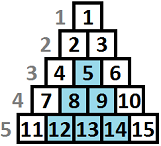
\includegraphics[width=0.5\textwidth]{fig354d_1.png}
				\caption{金字塔}
			\end{figure}
			
			可以按格式输出命令执行如下两种操作。①修改一个格子的值。格式:“1 格子编号 格子新值”。②修改一个子金字塔内所有格子的值。格式:“2 金字塔顶格子编号 内部格子1新值 内部格子2新值 ……”。新值可以和原值相同。
			
			现在有$k$个给定格子需要被修改成新值,问输出的命令中最少包含多少个数即可把金字塔修改成指定的样子。$n,k \leq 10^5$。
		
		\myparagraph{算法讨论}
		
			问题的本质是:修改一个格子有代价3,修改一个子金字塔有代价(2+子金字塔规模),问最小花费多少代价可使要修改的格子都被修改过,不用修改的格子也可被修改过。
			
			显然如果已经对一个子金字塔进行了操作,就没有必要对这个子金字塔的内部再进行操作了。由此可设状态$f[i]$表示金字塔中,以第$N-i+1$行第一个格子为顶的子金字塔(如后图左)中,要修改的格子都被修改过,的最小花费。在这个子金字塔的右边界上取一个高度为$j$的点为顶做第二种操作(取高度为0意为不取),其它区域用第一种操作修改,可列转移方程
			
			$$ f[i]=\min_{j,k|k \geq i-j} f[k]+\frac{j(j+1)}{2}+2+3\sum_{p=k+1}^i S[p][j+1-(i-p)] $$
			
			其中$S[p][x]$表示金字塔中第$N-p+1$行第一格与最后一行第$p$格的连线上高度大于等于$x$的要修改的格子的个数。
			
			这样是$O(n)$的状态,$O(n^2)$的转移。可以多设一维状态,将转移优化到$O(1)$。现在设$f[i][j]$表示在$f[i]$表示区域的右下角减去一个边长为$j$的三角形所组成的新区域(如后图右)中,要修改的格子都被修改过的最小花费。(现在枚举的使用第二种转移的子金字塔的顶的高度用字母$k$表示)有
			
			$$ \begin{aligned}
				f[i][0] = & \min_k f[i-1][k-1]+\frac{k(k+1)}{2}+2+3 S[i][k+1] & 0 \leq k \leq i \\
				f[i][j] = & \min(f[i][j-1],f[i-1][j-1]+3 S[i][j+1]) & j>0
			\end{aligned}$$
			
			\begin{figure}[ht]
				\centering
				\begin{minipage}{.45\textwidth}
					\centering
					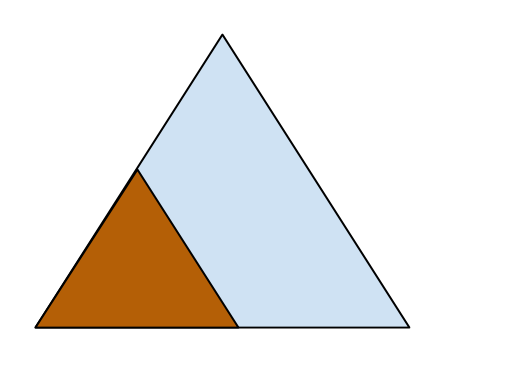
\includegraphics[width=\textwidth]{fig354d_2.png}
					\caption{f[i]表示的区域(橙色)}
				\end{minipage}
				\begin{minipage}{.45\textwidth}
					\centering
					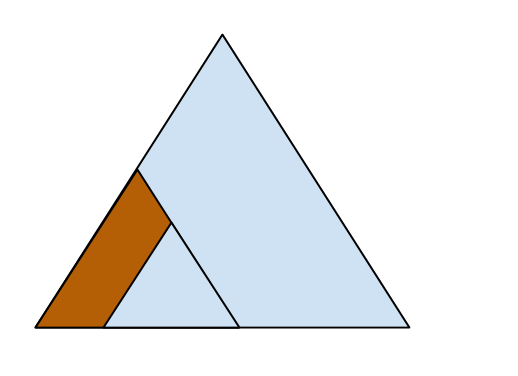
\includegraphics[width=\textwidth]{fig354d_3.png}
					\caption{f[i][j]表示的区域(橙色)}
				\end{minipage}
			\end{figure}
			
			这样是$O(n^2)$的状态,$O(1)$的转移。另外注意到$k$如果大于$\sqrt{6N}$没有意义,因为这样单次操作的花费就比把所有格子一个一个修改的花费还要高了,这样就可以把状态优化到$O(n^{1.5})$。
			
			另外$O(n^{1.5})$的状态需要$O(n^{1.5})$的空间,还需要优化空间。我们可以用滚动数组把$f$所需空间优化到$O(n^{0.5})$,另外用预先排序或者使用平衡树(std::map)也可以把$S$所需空间优化到$O(n)$。
		
		\myparagraph{时空复杂度}
		
			总时间复杂度$O(n^{1.5})$,空间复杂度最优可以做到$O(n)$。
	
	\section{Codeforces 356E - Xenia and String Problem}
	
		\myparagraph{题目大意}
		
			如果字符串$s$被称为Gray串,当且仅当($s$中的字符从1到$|s|$编号)
			
			\begin{enumerate}
				\item $|s|$是奇数;
				\item 字符$s[(|s|+1)/2]$在$s$中只出现一次;
				\item $|s|=1$或子串$s[1...(|s|+1)/2-1]$和子串$s[(|s|+1)/2+1...|s|]$相同且都是Gray串。
			\end{enumerate}
			
			给定串$t$,对于所有$t$的子串$t'$,如果它是Gray串,那么得分$|t'|^2$。问最多改动$t$中一个字符的情况下,最大得分是多少。
			
			$|t| \leq 10^5$,$t$中都是小写字母。
		
		\myparagraph{算法讨论}
		
			注意到Gray串的长度只能是$2^k-1$($k$为整数),$t$中的Gray子串最多$O(n\log_2n)$个。首先按照题意$O(n\log_2n)$递推得出每个长度为$2^k-1$的$t$的子串是否是Gray串。这一步需要判断两字符串是否相同(条件3),可用后缀数组或哈希$O(1)$判断(当然需要预处理)。还需要判断中间的字符是否只出现了一次,这可以二进制压位记录$t$的某一段中出现了哪些字符,这可以$O(1)$判断。
			
			接着,讨论需要改变字符的情况。如果是改变串最中间的字符,只需满足更改后该字符还是只出现了一次(条件2)。如果更改的是两边的字符,由于只能更改一次,肯定是把一边的改成与之对称的另一边的字符,只要更改后两边都是Gray串即可。这需要找出两侧唯一不同的字符(如果有),可用后缀数组或哈希求两边串的LCP,然后可用之前处理出的$t$的Gray子串来判断。
			
			如果子串$l \sim r$原是Gray串,如果改了$l \sim r$间的字符,那么它的得分就没了,在$l$处标记$-(r-l+1)^2$,在$r+1$处标记$+(r-l+1)^2$。如果要改字符,就统计把$x$位置改成字符$y$一共会增加多少得分。从小到大扫描坐标,统计标记的前缀和(减少的得分),加上该位置被修改成其它字符增加的得分,再加上原本就是Gray串带来的得分,对此求最大值即可。
		
		\myparagraph{时空复杂度}
		
			时间瓶颈在判断是否更改一个字符后可行。这需要先$O(|t\log_2|t|)$枚举候选串,然后需要$O(|\Sigma|)$的时间($\Sigma$表示字符集)的时间枚举换成什么字符(仅在改变最中间的字符时需要词枚举),总时间$O(|t| \cdot \log_2|t| \cdot |\Sigma|)$,总空间$O(|t|\log_2|t|+|t||\Sigma|)$。
	
	\section{CodeJam 2009 Finals B - Min Perimeter}
	
		\myparagraph{题目大意}
		
			给你一个整数坐标的点集,询问点集中最小的三角形周长是多少。退化的三角形也是允许的(面积为0)。共$n$个点,$n \leq 100000$。
			
		\myparagraph{算法讨论}
		
			这题的做法和求平面最近点对类似,用分治算法。可以把这些点按横坐标分为左右两部分,答案三角形可能在左边,可能在右边,也可能横跨左右。递归下去,即可解决前两种情况。对于每个子问题,先递归下去,假设这时已经找到的最小周长的三角形周长为$p$,再考虑横跨的情况。假设分割左右部分的竖直直线横坐标为$x_0$,显然我们只需考虑横坐标在$(x_0-p/2,x_0+p/2)$范围内的点,因为不在此范围内的点形成的横跨左右的三角形周长显然大于$p$。出于同样的原因,我们考虑的三角形的上下跨度也不应该超过$p/2$。
			
			因此我们可以维护一个区域,横坐标范围为$(x_0-p/2,x_0+p/2)$,纵坐标范围是$(y_0-p/2,y_0]$,我们只需考虑这个区域内的点。从小到大枚举$y_0$,每次加入纵坐标更大的一个点到这个区域中,枚举区域中的其它两个点与这个点组成三角形,判断是否能更新答案。一旦更新了答案$p$的值就会缩小,需要考虑的点的数目也会更小,而且因为读入的点一定是整点,此区域中的点的数目是非常有限的,可以认为是常数。用一个队列维护这个区域内的点。
			
			为了实现这个算法,我们需要在一开始对点按横坐标排序已进行左右分治,而合并左右时,则需按纵坐标扫描。因此,我们可以在执行分治的同时,执行归并排序算法。这样维护有序在整个算法中的总耗时就能保持在$O(n\log_2n)$。每次问题规模减少一半,若解决一个规模为$n$的子问题用时$f(n)$,$f(n)=2f(n/2)+n$,分治本身也是$O(n\log_2n)$的。
			
		\myparagraph{时空复杂度}
		
			时间$O(n\log_2n)$,空间$O(n)$。
	
	\section{CodeJam 2009 Finals D - Wi-fi Towers}
	
		\myparagraph{题目大意}
		
			平面上有$n$座信号塔($n \leq 500$),分别在位置$(x_i,y_i)$。每座塔有一个半径为$r_i$的圆形辐射范围。每座塔可以升级,收益$s_i$(正负皆有可能)。如果一座塔升级了,在它辐射范围内的所有塔都应升级。求最大总收益。有$T$组数据,$T \leq 55$。
		
		\myparagraph{算法讨论}
		
			建一张图,如果塔$a$升级了塔$b$就必须升级就从$a$向$b$连一条有向边,那么此问题就是一个典型的最大权闭合子图问题。解法是,使用网络流,设原点$s$和汇点$t$,对于所有$s_i$为正的点,连接有向边$s \to i$,容量为$s_i$;对于所有$s_i$为负的点,连接有向边$i \to t$,容量为$-s_i$;对于上述所有边$(a,b)$(塔的依赖关系),容量无限大。答案等于所有大于零的$s_i$之和减去此网络的最大流。此算法正确性可用最小割理解。
		
		\myparagraph{时空复杂度}
		
			网络中点数$O(n)$,边数$O(n^2)$。使用Dinic算法时间复杂度$O(\mbox{点数}^2\mbox{边数})$,故总时间$O(Tn^4)$。总空间$O(n^2)$。
	
	\section{CodeJam 2009 Finals F - Lights}
	
		\myparagraph{题目大意}
		
			有一个100×100的房间,里面有一个红色的点光源和一个绿色的点光源,还有$n$个大小不一定相同的圆($n \leq 50$),圆不透明。所有的圆之间相离,而且与房间的墙壁相离。给定光源的位置、圆的位置和圆的半径,要求输出整个房间里分别有多少面积无光、有红光、有绿光、有黄光(绿光+红光)。有红光或绿光的区域不包括有黄光的区域。
		
		\myparagraph{算法讨论}
		
			\subparagraph{(1)}
			首先独立地考虑两个光源照射到的区域,求出有哪些区域能被绿光源照到,哪些区域能被红光源照到。(包括被黄光照到的部分)
			
			即当前考虑的光源为$(x_0,y_0)$,先求出每个圆$(x-x_c)^2+(y-y_c)^2=r^2$过其的切线。可以设切线为$l:y-y_0=k(x-x_0)$,整理为$l:ax+by+c=0$,解方程$\frac{|ax_c+by_c+c|}{\sqrt{a^2+b^2}}=r^2$得斜率$k$。此处$k$无意义时应特殊处理。用斜率求出切线的极角(每条切线对应相差180度的两个角度),添加上房间四角的极角,按角度排序。这样每个角度对应一条从光源出发的射线,将房间分成若干部分。
			
			扫描每个部分。一个部分的边界即两条射线。枚举每个圆,找出最近的同时与两条射线不相离的圆,此圆即光在此部分能照到的最远处。如果没有这样一个圆,则光一直能照到墙壁。将此部分中能被光照到的部分分离出来:如果最远端是圆,则其为由两条线段和一条弧边构成的图形;如果最远端是墙壁,则其为一个三角形。对于第一种情况,我们可以简单地连接圆与射线的两个切点/交点,将此图形转化为三角形以便后续处理。为了判断圆与射线的位置关系并求出交点/切点,可以用参数方程表示切线:$(x=x0+p \cdot \Delta x, y=y0+p \cdot \Delta y)$。$(\Delta x, \Delta y)$为射线的方向向量。解方程$(x0+p \cdot \Delta x-x_c)^2+(y0+p \cdot \Delta y-y_c)^2=r^2$即可。
			
			至此,我们分别对于两个光源,把它能照到的区域分成了若干个三角形。
			
			\subparagraph{(2)}
			现在我们要计算这些三角形的交以求出被黄光照到的区域。枚举每一对三角形,求它们的交——一个凸多边形。把两个三角形的六个顶点和最多九对边的交点放在一起,找出其中的被两个三角形同时包含的点,去掉重复,就是构成交的多边形的顶点。对这些顶点排序,即可得三角形的交。
			
			\subparagraph{(3)}
			最后统计面积。我们需要知道以下三个区域的面积:所有被红光源照到的区域(包括黄光的部分),所有被绿光照到的部分(也包括黄光),所有被黄光照到的部分。
			
			前面我们已经把所有要统计面积的部分分割为了若干凸多边形(包括三角形),但其中一部分面积可能被圆覆盖。扫描每个多边形,如果它与任何一个圆都没有交,直接计算它的面积即可,否则一个多边形最多只能和一个圆有交,并且和圆的交点一定是多边形的顶点之一,这从上面求多边形的过程可以看出。将此多边形与圆的两个交点连起来,将多边形分成两半,去掉在圆内的一半。计算剩余一半的面积记作$S1$,求出两个交点与圆心构成的扇形的面积记为$S2$,再求出两个交点与圆心构成的三角形的面积$S3$,实际面积为$S1-S2+S3$。依次求出总面积。
			
			最后根据求出的这三个区域的面积求出题目要求的四个面积即可。
		
		\myparagraph{时空复杂度}
		
			此算法分若干步。上文的(1)部分需扫描每个圆求出切线、对切线排序、对每个切线再扫描每个圆,最后一项为瓶颈,时间复杂度$O(n^2)$。(2)部分需扫描每对三角形,再求交,求交的复杂度与多边形边数(不超过5)有关,可认为是常数,时间复杂度$O(n^2)$。(3)部分需枚举$O(n^2)$个多边形,再枚举每个圆,时间复杂度$O(n^3)$。总时间复杂度$O(n^3)$。所有$O(n^2)$个三角形交不用都存下来,可以算出一个就计算一个的面积,其余所有存储的空间需求都是$O(n)$的。总空间复杂度$O(n)$。
	
	\section{CodeJam 2010 Finals A - Letter Stamper}
	
		\myparagraph{题目大意}
		
			有一个栈,每次操作可以往里加入一个字母,或者从中弹出一个字母,或者打印栈顶的字母。给一个字符串$S$($|S| \leq 2000$),要求操作中打印出的序列就是这个字符串,还要求栈一开始是空的,最后也是空的,问最小操作次数。$T$组数据$T \leq 20$。字母只有‘A’、‘B’、‘C’三种。
		
		\myparagraph{算法讨论}
		
			设已经做了一下操作,现在栈顶部的三个字母从下往上分别是$X$、$Y$、$Z$。假设下一个要打印的字母是$Z$,显然直接打印栈顶是最优的。如果下一个要打印的是$Y$,删除栈顶的$Z$比加入一个新的$Y$优,因为后者会增加最后把栈清空的代价,而其它影响都相同。如果下一个要打印的字母是$X$,可以选择删除$Z$和$Y$,也可以选择加入一个$X$。这样,栈中的排列就只可能是每三个字母一次循环,如“ABCABCABC”或“BACBACBAC”。只有六种情况。
			
			设状态$f[i][j][k]$表示目前已打印$i$个字母,栈中的排列是第$j$种情况(共六种),栈中共$k$个元素的最小操作次数。按上面的规则直接转移即可。
		
		\myparagraph{时空复杂度}
		
			DP状态$O(|S|^2)$,每次转移$O(1)$。总时间$O(T|S|^2)$,总空间$O(|S|^2)$。
	
	\section{CodeJam 2011 Finals A - Runs}
	
		\myparagraph{题目大意}
		
			给定一个仅包含小写字母的字符串$S$($|S| \leq 450000$),$S$中每一段连续的相同字符称为一个run,比如“abba”中有“a”、“bb”、“a”三个runs。问如果把$S$的字符重排,能有多少种方案的run数目和原来一样多。给定$S$的run数目不超过100。有$T$组数据。
		
		\myparagraph{算法讨论}
		
			从'a'到'z'依次考虑26个字母来DP。设状态f[i][j]表示当前已经考虑了$i$个字母,组成$j$个run的方案数。每次我们要把所有字母$i$都插入到已构建的字符串中,这只有两种情况:要么插入到两个run之间,使run数目增加1;要么插入到一个run中,把这个run分成两个runs,run数目共增加2。
			
			枚举有$p$个新run被插入到原来两个run之间,有$q$个新run被插入到原来的一个run中,那么插入前一共有$j-p-2q$个run。记字母$i$共有$num_i$个,$i$及$i$之前的字母共$sum_i$个。这样就共有$j-p-2q+1$个位置可供第一种插入用,共$(sum_{i-1}+1)-(j-p-2q+1)=sum_{i-1}-j+p+2q$个位置可供第二种插入用。选择插入位置共$\binom{j-p-2q+1}{p}\binom{sum_{i-1}-j+p+2q}{q}$种方案。另外还需要把当前的$num_i$个$i$分配到$p+q$个新run中,共$\binom{num_i-1}{p+q}$种方案。综上
			
			$$ f[i][j]=\sum_{p,q} f[i-1][j-p-2q] \cdot \binom{j-p-2q+1}{p}\binom{sum_{i-1}-j+p+2q}{q}\binom{num_i-1}{p+q} $$
			
			$f['z'][\mbox{原run数目}]$即为答案。预处理组合数,直接转移即可。DP时要注意判断$p$、$q$是否使转移合法。
		
		\myparagraph{时空复杂度}
		
			记字符串长$L$,有$n$个run,字母数$|\Sigma|$,共$T$组数据。预处理组合数:时间$O(Ln)$,空间$O(Ln)$。DP:时间$O(T |\Sigma| n^3)$,空间$O(|\Sigma| n)$。
	
	\section{CodeJam 2011 Finals B - Rains Over Atlantis}
	
		\myparagraph{题目大意}
		
			你有一幅地图。地图是一个矩形的网格,每个格子里有一个整数表示该位置海拔为多少米。网格外面是大海,海拔为零。所有为海拔零的格子都是水域,所有海拔大于零的格子都是陆地,没有海拔小于零的区域。
		
			如果两个格子有公共边,水就能从高的格子流向低的格子。如果两个有公共边的格子一样高,水能向任意一边流。
		
			正在下大雨,所以如果一个格子里的水流不走,就会积在那里,直到水平面足够高使其得以流走。地图外面的大海可以接收任意多的水。举个例子,比如下面这幅地图:
		
			\begin{center}\fbox{\shortstack{5 9 9 9 9 9 \\ 0 8 9 0 2 5 \\ 3 9 9 9 9 9}}\end{center}
		
			低洼地区会积水。我们把积水地区的海拔加上水深称为\emph{水平面},上面地图的水平面将会是:
		
			\begin{center}\fbox{\shortstack{5 9 9 9 9 9 \\ 0 8 9 \textbf{5 5} 5 \\ 3 9 9 9 9 9}}\end{center}
		
			注意中间地域的0,尽管它是水域,因为它不与外界相连,所以它也会积水。边界上的0与外界相连,所以来自8的水可以经它流走。
		
			水流动的方向决定于水平面的高低。如果与一个区域相邻(有公共边)有若干个区域的水平面都比它低,那么它的水就会流向其中最低的一个。如果最低的也有多个,流向哪里没有所谓,这在下文会提到。
		
			现在流水侵蚀开始了。每天,一个格子被侵蚀掉多少——海拔降低多少——决定于水怎么流过它。如果水从S流到与S相邻的T,那么S的海拔将降低min(S的水平面-T的水平面,M)。所有的侵蚀都在同一时间——一天结束的时候——发生。例如,M=5时,上面的地图描绘的土地就会被侵蚀成下面这个样子:
		
			\begin{center}\fbox{\shortstack{0 4 4 4 4 4 \\ 0 3 5 0 2 0 \\ 0 4 4 4 4 4}}\end{center}
		
			一天的侵蚀过后,多余的水会流走:当一片区域的水平面高于与它相邻的区域的水平面时,水就会从高处流到低处,直到两个区域水面相平。水依然回像第一天那样积累。第二天,水平面变成:
		
			\begin{center}\fbox{\shortstack{0 4 4 4 4 4 \\ 0 3 5 \textbf{2} 2 0 \\ 0 4 4 4 4 4}}\end{center}
		
			又过了一天的侵蚀,地图又变成下面这样:
		
			\begin{center}\fbox{\shortstack{0 0 0 0 0 0 \\ 0 0 2 0 0 0 \\ 0 0 0 0 0 0}}\end{center}
		
			计算要过多少天亚特兰蒂斯的海拔高度会全变成0。
			
			共T组数据。1≤T≤10, 1≤H,W≤20, 1≤M≤$10^{15}$, 0≤所有海拔≤$10^{15}$。
			
		\myparagraph{算法讨论}
		
			算法核心是模拟,但海拔高度很大而M很小时直接模拟就不能解决问题了,所以我们需要同时计算多天的侵蚀。当下列条件同时满足,就可以同时计算多天:
		
			\begin{itemize}[leftmargin=15mm]
				\item 所有未被淹没的格子都以最大速度被侵蚀。
				\item 所有的水面都在以最大速度下降。
				\item 未出现被淹没的格子露出水面的过程。
			\end{itemize}
		
			像下面这样同时计算多天:
		
			\begin{enumerate}[leftmargin=15mm]
				\item 计算每个格子的水平面。
				\item 判断每个未被淹没的格子是否以M的速度被侵蚀,如果不是就只计算一天。\textbf{注意我们可以让格子的海拔降到负数},即假定地图外的海拔是无穷小,这样不会改变结果,并会大大简化问题。
				\item 如果每个未被淹没的格子都是以M的速度被侵蚀,那么每个“湖”的水平面也会以M的速度下降。因为一个“湖”是由至少一个在湖边上未被淹没的格子决定高度的,而这个格子的高度正以M的速度下降。所以某些被淹没的格子露出水面之前的侵蚀都可以一起计算。
				\item 由此我们找出被淹没格子水深的最小值,就可以算出有多少天可以一起计算。
				\item 如果没有任何一个格子在水下,就还剩$\lceil \mbox{最高海拔}/M \rceil$天就侵蚀完了。
			\end{enumerate}
		
			注意每次同时计算后都会有一个被淹没的格子露出水面,而显然露出水面的格子不会再被淹没,所以最多执行$HW$次同时计算。(事实上这个数字会更小,因为地图边缘的格子不会被淹没)
		
			现在我们就要算出最多要经过多少次普通的一天一天地计算后,才能进行同时计算。定义一个辅助的图来进行说明:每个未被淹没的格子对应图上的一个节点,每个“湖”的所有格子对应图上的一个高度为“湖”的水平面的节点。节点S和节点T间有连边当且仅当S对应的任意一个格子与T对应的任何一个格子有公共边。称一个节点的父节点为与其相邻的高度最低的节点。这样我们就有了一棵根在外海中的树。我们定义一条向海拔高的方向走的的树上路径为确定路径,当且仅当这条路径上每条边的高度差都为M。我们能证明每天过后都能发生如下的事件之一:
		
			\begin{itemize}[leftmargin=15mm]
				\item 有被淹没的区域露出水面了(这样执行同时计算的次数就会减少)
				\item 确定路径上节点增多了
				\item 所有的节点都在确定路径上了
			\end{itemize}
		
			原因如下:考虑任意一条确定路径。假设节点的分布维持不变(即陆地还是陆地,湖还是湖),这条路径在一天后还是确定路径,因为其上的每个节点都在以M的速度降低。考虑任意一个不在确定路径上但它父节点在确定路径上的节点(注意前面为了方便把海平面定义为无穷低,海平面在确定路径上,如果不存在这样的节点,那么所有节点都在确定路径上了),一天后此节点的高度降到了它父节点的高度,而它父节点的高度下降了M,所以现在它和它父节点的高差也变成了M,它也加入了确定路径。
		
		\myparagraph{时空复杂度}
		
			如果所有的节点都在确定路径上,我们就能进行同时计算了。每次同时计算前最多有$HW$次路径上节点的增多,这样每一个被淹没的格子露出水面前最多有$HW$次普通计算和一次同时计算,总计$(HW)^2$次普通计算和$HW$次同时计算,总时间复杂度为$O(T(HW)^3 \log_2(HW))$,空间复杂度$O(HW)$。
	
	\section{CodeJam 2011 Finals C - Program within a Program}
	
		\myparagraph{题目大意}
		
			你需要构造一个图灵机,满足如下要求:此图灵机有一个无限长的纸带,纸带上有格子(原题是路旁的路灯),格子的编号自西向东递增,每个格子里有一个绝对值$10^6$以内的数。每时每刻图灵机内部有一个绝对值$10^6$以内的整数状态,并且有一个指针指向纸带上的某一格。图灵机有不超过$30$条执行规则,每条形如“$<S> <M> \to <\mbox{操作}>$”。表示当内部状态为$S$且指针指向的格子里的数为$M$时怎么做,$<$操作$>$有如下两种:
			
			\begin{enumerate}
				\item “$<D> <NS> <NM>$”,表示指针向方向$D$移动一格(E为东,W为西),内部状态变为$NS$,指针原来指向的格子里的数变成$NM$。
				\item “R”,表示结束程序。
			\end{enumerate}
			
			图灵机初始时纸带上所有格子中的数都是0,指针指向第0格,内部状态为0。对于读入的$N$,你需要输出图灵机的规则使其在执行不超过1.5×$10^5$步后程序结束,并且结束时指针恰好在第$N$格。
		
		\myparagraph{算法讨论}
		
			如果没有规则数上限$30$,一个显而易见的做法是在内部状态中记录还有多少步要走。构造如下规则:
			
			\begin{verbatim}
				<0> <0> -> <E> <1> <0>
				<1> <0> -> <E> <2> <0>
				……
				<N> <0> -> R
			\end{verbatim}
			
			但这样需要$N$条规则。但是剩余步数不仅可以记录在内部状态中,我们把剩余步数以二进制的形式从高位到低位记录在纸带上,末位在第0格。用1和2表示原二进制中的0和1。这样我们只用连续执行以下两个子程序直到这个数字为0:
			
			\begin{enumerate}
				\item 做二进制减法将这个数减一。具体地,从东向西扫描,将末尾连续的1变为2,把接下来的一个2变为1,剩下的数字不变,但仍要把指针移到最西侧以便做下一步操作。用内部状态标记当前的数字应变化还是不变。此步在遇到0时停止。
				\item 将这个数向东平移一格。具体地,从西向东扫描,在内部状态中记录上一个数是多少,在当前格写入这个数字。此步在遇到0时停止。
			\end{enumerate}
			
			当这个数字为0时指针的位置就是第$N$格(因具体实现不同,可能有一或两格的偏移,需手动修正)。
		
		\myparagraph{图灵机规模}
		
			本题要提交的程序时间复杂度$O(\log_2N)$,空间复杂度$O(1)$,但我们关心的主要是图灵机的规模。只要实现时不太浪费,节约要用到的内部状态数,规则数就能控制在$30$以内。因为数字总共要平移$N$格,数字长$\log_2N$,每次移动需扫描这个数两边,总步数大约$2N\log_2N$。向东平移时,需去掉前导零以减短数字长度,这样就可以将总步数控制在1.5×$10^5$内。
	
	\section{CodeJam 2012 Finals D - Twirling Towards Freedom}
	
		\myparagraph{题目大意}
		
			平面上有$N$个点,一开始你在原点,每次能选一个点,以它为中心顺时针旋转90度,最多旋转$M$次。问你最远能到达离原点多远的地方。有$T$组询问。(1≤$N$≤5000, 1≤$M$≤$10^8$, $T \leq 100$)
		
		\myparagraph{算法讨论}
		
			将点画在复平面上,记这些点为$p_j=a_j+b_j\mathrm{i}$,记你所在的点为$z=x+y\mathrm{i}$。绕点$j$旋转90度后$z'=-(z-p_j)\mathrm{i}+p_j=-z\mathrm{i}+p_j(1-\mathrm{i})$。设共旋转$m$次($m \leq M$),第$j$次旋转的中心为$q_j$($0<j \leq m$),带入并展开上式得最终位置
			
			$$z"=(1-\mathrm{i})\sum_{j\mod 4=0}q_{m-j}+(-1-\mathrm{i})\sum_{j\mod 4=1}q_{m-j}+(-1+\mathrm{i})\sum_{j\mod 4=2}q_{m-j}+(1+\mathrm{i})\sum_{j\mod 4=3}q_{m-j}$$
			
			显然对所有$j\mod 4$相同的$q_j$应取相同的点。将所有的$p_j$分别乘上$(1-\mathrm{i})$、$(-1-\mathrm{i})$、$(-1+\mathrm{i})$和$(1+\mathrm{i})$后建四个凸包。在这四个凸包上扫描一个方向,求出在这个方向上四个凸包分别对应的离圆心最远的点,这四个点对应的复数乘上系数后的和即为上述$z"$,求出其最大模长即为答案。从上式看出此系数与$m$相关,显然$M-3 \leq m \leq M$,枚举$m$即可。
		
		\myparagraph{时空复杂度}
	
			枚举$m$时间$O(4)=O(1)$,建凸包时间$O(N\log_2N)$,扫描时间$O(N)$。考虑数据组数$T$,总时间复杂度$O(TN\log_2N)$,空间复杂度$O(N)$。
	
	\section{CodeJam 2013 Finals A - Graduation Requirements}
	
		\myparagraph{题目大意}
		
			有一个有$N$个出口的环岛,从时刻0到时刻$X$观察,有$C$辆车通过。每辆车在对应的某时刻进入环岛,每过单位时间到达下一个出口,并在某时刻离开环岛(不会转满一圈)。假如要选一个0到$X$间的时刻进入环岛,并在环岛上以每单位时间一个出口的速度逆行,要求不能与其它车会车,可以在$X$时刻前的任一时刻离开环岛,问最多能在环岛上转多久(可以转一圈以上)。须在整数时刻进入环岛。$X,N \leq 10^{10}$,$C \leq 1000$。有$T$组数据。
		
		\myparagraph{算法讨论}
		
			建立坐标系,横坐标为出口,纵坐标为时刻。横坐标是循环的,即认为$x=x_0$与$x=x_0+N$是相同的横坐标。问题转化为,在坐标系上找出最长的斜率为-1的端点为整点的线段$l$(当然要在0到$X$范围内),不与某些斜率为1的线段$a_i$相交。不失最优性,可以认为$l$过与$a_i$的端点相距1单位(或2,后述)的整点,因为对于任意一个最优的$l$,都可以将其平移至这样一个位置,如图:
			
			\begin{figure}[ht]
				\centering
				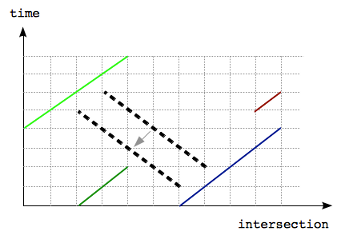
\includegraphics[width=0.8\textwidth]{figgcj2013a_1.png}
				\caption{相距1单位}
			\end{figure}
			
			不过也有特殊情况,这种情况要求我们也考虑与$a_i$的端点横纵坐标都差1的点。如图:
			
			\begin{figure}[ht]
				\centering
				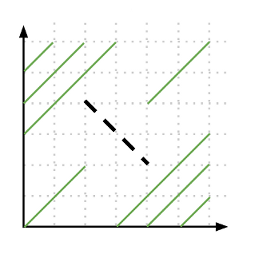
\includegraphics[width=0.6\textwidth]{figgcj2013a_2.png}
				\caption{相距2单位}
			\end{figure}
			
			接下来,枚举这些“必经点”,计算如果线段$l$经过它最多能延伸多长。枚举$a_i$,我们先求直线$l$与它最近的一个(或两个,在两个方向上)的交点在哪,再据此求出其附近最近的一个$l$上的整点。但因为横坐标是循环的,所以略微繁琐。首先求出直线$l$与它任意一个交点的纵坐标$t$(不必最近,也不必为整数),这可以直接解方程得到。注意到所有交点的纵坐标都可以表示为$t+\frac{1}{2}kN$($k$为整数)。接下来确定有用的$k$的范围,记$a_i$起点和终点的纵坐标分别为$T_i$和$R_i$,$\frac{T_i-p}{N} \leq k \leq \frac{R_i-p}{N}$。$k$最多有两种取值,枚举$k$,算出对应交点,再算出最近的整点,更新对$l$的限制,最后取最紧的限制即可。
		
		\myparagraph{时空复杂度}
		
			枚举$a_i$确定必经点,再枚举$a_i$确定$l$最多能延伸多长,其中的每次计算虽然情况很多,但都是线性的。总时间$O(C^2)$,总空间$O(C)$。
	
	\section{CodeJam 2013 Finals C - X Marks the Spot}
	
		\myparagraph{题目大意}
		
			平面上有$4N$个点($N \leq 2500$),要求作两条相互垂直的直线,把平面分为四个部分,每个部分点数一样多。输出任意方案。任意三点不共线。
		
		\myparagraph{算法讨论}
		
			如果这两条直线都是平行于坐标轴的,记这$4N$个点在$x$轴和$y$轴上的中位数分别为$x_M$和$y_M$,则显然这两条直线应分别为$x=x_M$和$y=y_M$。对于一般情况,可以将整个平面逆时针旋转$\alpha$角,就转化成上面的情况。
			
			先不考虑有点恰好在$x=x_M$或$y=y_M$上的情况,检验这种方案是否合法:以$x=x_M$和$y=y_M$为轴建新坐标系$y'-x'$,如果没有点落在坐标轴上,记其第一象限有$X$个点,则第二象限有$2N-X$个点,第三象限有$X$个点,第四象限有$2N-X$个点。如果$X=N$,那么此方案就合法了,否则要调整这个坐标系。
			
			如果将这个坐标系顺时针旋转$90^\circ$,那么第二象限变为第一象限,第三象限变为第二象限……旋转过程中,第一象限中点数逐渐由$X$变为$2N-X$,其中肯定会经过$N$(因为任意三点不共线,不考虑点恰好落在坐标轴上的情况,每次$X$最多变化1)。因此可以二分这个位置。先判断$X$是大于$N$还是小于$N$以确定二分时的调整方向,然后在$0^\circ \leq \alpha \leq 90^\circ$上二分这个使$X=N$的$\alpha$。
			
			如果在某个$\alpha$处有点正好落在坐标轴上,那么第二象限和第四象限的点数就不再是$2N-X$,不再可以直接比较$X$和$N$的大小关系。但是既然总点数是偶数,任意三点又不共线,一条坐标轴上最多有两个点,只要将这两个点分别计入两侧的象限依然不影响比较,显然这样判定出的二分调整方向仍然是正确的。事实上,这等价于直接比较第一象限和第二象限点数的大小关系。当然,最后输出的解不能导致点在坐标轴上的情况,但是这种情况非常稀少,不在$0^\circ \leq \alpha \leq 90^\circ$上二分而是初始一个随机角度$\theta$,在$\theta \leq \alpha \leq \theta+90^\circ$上二分即可。
		
		\myparagraph{时空复杂度}
		
			二分复杂度与是对数级别的,记为$log$,每次二分需要$O(N)$做快速查找找出中位数,总时间复杂度$O(log \cdot N)$。总空间复杂度$O(N)$。
	
	\section{CodeJam 2014 Finals C - Symmetric Trees}
	
		\myparagraph{题目大意}
	
			给一棵$N$个节点的树($N \leq 10000$),每个节点有一个颜色(颜色最多26种),现在问它是不是对称的。对称的定义是,能把这棵树放在一个平面上,$x=0$为对称轴,若在$(x,y)$处有一点$v$,那么在$(-x,y)$处就一定有一个相同颜色的点$v'$(如果$x=0$则它们为同一点),并且对于所有边$(u,v)$,$u'$和$v'$间也一定有边。共$T$组数据,$T \leq 100$。
	
		\myparagraph{算法讨论}
		
			分两种情况。如图(图片可能在下一页):
			
			\begin{figure}[ht]
				\centering
				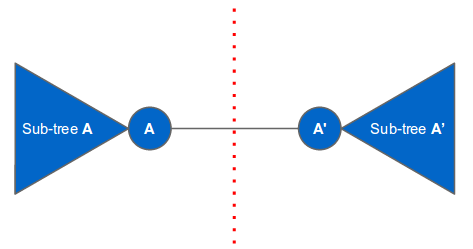
\includegraphics[width=0.8\textwidth]{figgcj2014c_1.png}
				\caption{情况1}
			\end{figure}
			
			\begin{figure}[ht]
				\centering
				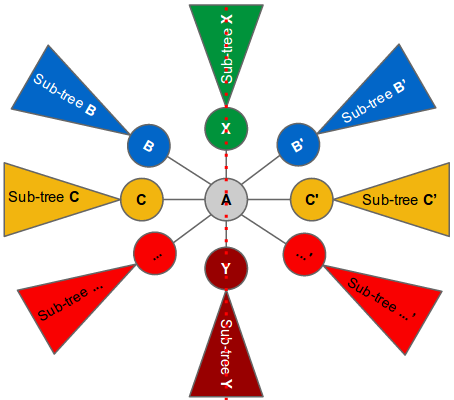
\includegraphics[width=0.8\textwidth]{figgcj2014c_2.png}
				\caption{情况2}
			\end{figure}
		
			即:
		
			\begin{enumerate}
				\item 如果对称轴上没有点,那么树一定能分成两个互相同构的子树。
				\item 否则对称轴上有若干点。任取其中一点,考虑所有以它为根的子树,分为两种。一是图中的$(B,B')$、$(C,C')$等,成对出现,每对相互同构;二是图中的$X$和$Y$,它们本身就是对称的,而且最多只能有两个。
			\end{enumerate}
			
			为了计算两棵子树是否同构以及每棵子树本身是否对称,枚举所有$2N-2$棵子树,计算它的哈希值。为了对树做哈希,我们可以把树看作一个字符串,对其做先序或后序遍历,并用特殊字符标志其中每棵子树的范围,这样即可使用字符串哈希的方法哈希。为了保证以一个节点的子节点为根的子树之间是无序的,需先对这些子树按其哈希值大小排序再进行遍历。当然,为了保证线性时间,要使用记忆化,即对于每个节点,用以其子节点为根的每棵子树的哈希值计算出以该点为根子树的哈希值,而不是每次都重新遍历。CodeJam数据较强,没有依据地随便哈希是不能得出正确答案的。
			
			为了判断一棵子树本身是否对称,将其下(以这棵子树的根的子节点为根的,下同)的互相同构的子树配对,如果所有子树都能配对或者剩下的最多一棵子树本身也是对称的,那么它就是对称的。配对在上文所述排序后扫描即可实现。
			
			最后,如果是第一种情况,直接判断是否存在一条边两侧的的子树哈希值是否相同即可;否则枚举一个点,以它为根,将其下子树按哈希值排序后配对,并检验未配对的子树的对称性即可得出答案。
		
		\myparagraph{时空复杂度}
	
			预处理所有子树的哈希及其本身的对称性时,需枚举所有$2N-2$棵子树,并对其下所有子树按哈希值排序,考虑上数据组数,总时间复杂度$O(TN\log_2N)$。总空间复杂度$O(N)$。
	
	\section{CodeJam 2014 Finals D - Paradox Sort}
	
		\myparagraph{题目大意}
		
			有$n$个糖果($n \leq 100$),对于每对糖果,Vlad都更喜欢其中的一个,但是它的偏好不一定满足偏序关系。你要按一定顺序依次给他$n$个糖果,每时每刻Vlad只拿着一颗。每次如果相比手上的,他更喜欢新的,它就扔掉手上的拿新的,否则不拿新的。你要设计一个这样的顺序,使他最后拿着的糖果编号为$A$,如果有多解输出字典序最小的顺序。有$T$组数据,$T \leq 100$。
		
		\myparagraph{算法讨论}
		
			首先我们要能判断是否有解。对于每一对糖果$(x,y)$,如果Vlad更喜欢$x$,就连一条$x$到$y$的边,否则连一条$y$到$x$的边。以$A$为根,DFS遍历整个图,如果所有点(糖果)都被遍历到了,那么有解,否则无解。
			
			\begin{proof}\mbox{}\\
			
				如果所有点都被遍历到了,可以构造一棵DFS树,此树的后序遍历就是一个合法解。原因如下:记当前遍历到$y$点,手上拿着的糖果是$x$点,$x$肯定被遍历过。如果$x$是已经遍历过的点中深度最浅的,按照后序遍历的特点,$y$最浅的可能深度也只能比$x$的深度小1,而且此时必然有边$y \to x$,Vlad会扔掉$x$拿$y$,手上拿的仍然是深度最浅的一个。而一开始只有一个点被遍历过时,$x$必然是最浅的一个。所以最后Vlad拿着的一定是根节点对应的糖果。
				
				如果有点没被遍历到,假设该点为$p$。对于能遍历到的部分任意点$q$,都有边$q \to p$。如果给Vlad遍历过的点,再给$p$,他就一定会拿$p$;反之先给$p$,它就永远拿不到遍历过的点,包括$A$。
				
			\end{proof}
			
			下一步我们要求字典序最小。因为是字典序,如果前面的糖果编号大了,后面的糖果编号再小也没用,所以我们使用贪心。一个糖果一个糖果地构造答案序列。假设当前构造到第$i$个,从小到大尝试第$i$个是什么,如果加上此糖果就有解了,就用此糖果,继续做第$i+1$个,否则继续尝试更大编号的糖果。
			
			不过因为已经选了$i$个糖果了,判断是否有解的方法较上面更复杂。记给完这$i$颗糖果,Vlad手上拿着的是糖果$B$。分两种情况讨论。
			
			\begin{enumerate}
				\item 如果$A$在这$i$颗糖果中,假设$A \not= B$,显然无解。否则仅对于所有没给过的糖果$j$都有边$i \to j$的情况才有解。
				\item 否则,仍以$A$为根遍历,但不访问$B$,最后再把$B$和所有满足有边$B \to x$的点$x$加入DFS树。此树的后序遍历是合法解,理由类似上面。
			\end{enumerate}
			
		\myparagraph{时空复杂度}
		
			首先要枚举$i$,再$O(n)$枚举第$i$颗糖是什么,再$O(n)$遍历判断是否有解,考虑上数据组数$T$,时间复杂度$O(n^3T)$。空间复杂度为存图的空间复杂度,为$O(n^2)$。
	
	\section{CodeJam 2014 Finals E - Allergy Testing}
	
		\myparagraph{题目大意}
	
			Kelly对$N$种食物中的一种过敏,她要做试验找出到底对哪种过敏。每次她可以选一部分食物吃,等$A$天后如果没有过敏反应,则使她过敏的食物不在这一部分里,否则在,而且她还要继续等$B-A$天等反应消去才能进一步实验。为了实验的严谨性,必须等上一次试验结束之后(等了$A$天或$B$天)才能做下一次试验。给定$N$、$A$、$B$,问最少要花多少天Kelly才能确定对哪种食物过敏。$1 \leq N \leq 10^{15}, 1 \leq A \leq B \leq 10^{12}$。
	
		\myparagraph{算法讨论}
		
			用DP解决。一个显然的方法是用还需要试验的食物种数作状态,但这样最快只能优化到$O(N)$。按另一种思路,可以以剩余天数作状态,设$f[i]$表示用$i$天最多能试验多少食物,假设求得了$f$,即可二分答案出解。考虑转移方程:当前有$i$天时间,假设要先吃$x$种,还剩$y=f[i]-x$种。如果过敏了,就要等$B$天,然后要在$i-B$天内在这$x$种中确定过敏原;否则就要等$A$天,然后在$i-A$天内在$y$种中确定过敏原。为了使$x$和$y$尽量大,$x=f[i-B], y=f[i-A]$。所以转移方程为
			
			$$f[i]=x+y=f[i-A]+f[i-B]$$
			
			还要考虑边界状态。显然$f[i]=1$当且仅当$i<A$。另外如果$x=1$,吃完后即使过敏也不用等它消退,只用等$A$天。但如果$i-A \leq B \Leftrightarrow i-B \leq A$,那么$x=f[i-B]>1$更优,所以$x=1$只存在于$i-B<A$时,不妨仍把它写成$x=f[i-B]=1$,两者等价。所以总方程为
			
			$$f[i]=\left\{\begin{array}{ll}
				f[i-A]+f[i-B] & i \geq A \\
				1 & i<A \mbox{(此处允许负数)}
			\end{array}\right.$$
			
			这样的算法仍不能被接受,要继续优化。假设二分答案时我们二分到了$D$天,把DP的转移树画出来,根为$f[D]$,对于每个节点$f[i]$,$f[i-A]$和$f[i-B]$分别是它的两个子节点。$f[i]=1$的点为叶节点,$i<A$。$f[D]$等于整棵树上叶节点的个数。每个叶节点对应一条从根出发到它的路径,路径上的每条边要么是$-A$转移要么是$-B$转移。所以我们可以枚举总共有$i$个$-A$转移,$j$个$-B$转移,则
			
			$$f[N]=\sum_{D-A<iA+jB\leq D}\binom{i+j}{j}$$
			
			可以用树高估计数的规模,因为$B>A$,所以$f[N]>2^j \Rightarrow j<\log_2f[N]$,$j$最多只有60,所以可以枚举$j$。
			
			$$\begin{aligned}
				f[N]&=\sum_{j=1}^{60}\sum_{i=\lfloor \frac{D-jB-B}{A} \rfloor+1}^{\lfloor \frac{D-jB}{A} \rfloor} \binom{i+j}{j} \\
				    &=\sum_{j=1}^{60}(\binom{\lfloor \frac{D-jB}{A} \rfloor+j+1}{j+1}-\binom{\lfloor \frac{D-jB-B}{A} \rfloor+1+j}{j+1})
			\end{aligned}$$
			
			二分答案后直接计算此式就能出解。为了避免算术溢出,可以使用浮点数近似计算,也可以写高精度。
		
		\myparagraph{时空复杂度}
		
			二分答案$O(\log_2N)$,枚举$j$需$O(\log_2{f[N]})$,计算组合数需$O(j)=O(\log_2{f[N]})$。$\log_2{f[N]}<\log_2N$,所以$O(\log_2{f[N]})=O(\log_2N)$。总时间复杂度$O(\log_2^3{N})$。空间复杂度$O(1)$。
	
	\section{CodeJam 2014 Finals F - ARAM}
	
		\myparagraph{题目大意}
		
			游戏中有$N$个英雄($N \leq 1000$),你用其中每个玩一局都有一个相应的胜率$P_i$。现在你要玩$10^{100}$局,每局开始前要随机抽一个英雄用,如果对抽到的英雄不满意可以重抽,重抽依然是随机的。每次重抽要用一块钱,只要有钱就可以重抽任意次。最初有$R$块钱,每次玩完一局,不管输赢都能挣$1/G$块钱($R,G \leq 20$)。求期望赢的局数占总局数$10^{100}$的比例的最大值。有$T$组数据。
		
		\myparagraph{算法讨论}
		
			由于$10^{100}$很大,可以当作无限大考虑,这样每次决定是否重抽仅与当前剩余的钱数和抽到了什么英雄有关。显然剩余钱数相同时,使我们决定要重抽的英雄的胜率一定比使我们决定不重抽的英雄的要低,所以对于特定的剩余钱数,肯定是英雄胜率小于某临界值时就重抽,否则不重抽。
			
			我们要求的是赢的局数占总局数的比例,不便于处理,可以通过二分答案去除总局数的影响:设二分到的答案为$K$,再设$f[i]$表示目前剩余$i$块钱时,一直玩直到钱数大于$i$期间,胜利数相比二分出的答案多了(或少了)多少。$f[i]$表示的是总的胜利数,不用除总局数。
			
			$0 \leq i < 1$时,不能重抽,所以
			
			$$f[i]=\frac{1}{N}\sum_{j=1}^N(P_j-K)$$
			
			$1 \leq i < R$时,记如果抽到了胜率前$X_i$小的英雄要重抽,
			
			$$f[i]=\min_{X_i} \frac{X_i}{N}\sum_{j=0}^G f[i-1+\frac{j}{G}] + \frac{1}{N}\sum_{j=X_i+1}^N(P_j-K)$$
			
			$i=R$时,稍修改一下定义,$f[R]$是一直玩直到钱数再次等于$R$期间胜利数相比二分出的答案的盈余或亏损。
			
			$$f[R]=\min_{X_i} \frac{X_i}{N}\sum_{j=0}^{G-1} f[i-1+\frac{j}{G}] + \frac{1}{N}\sum_{j=X_i+1}^N(P_j-K)$$
			
			$f[R]>0$时,说明$K$小了;$f[R]<0$时,说明$K$大了。为什么?虽然这样算结束时还有$R$块钱,答案理应更大些,但是用完这$R$块钱能多出的胜率在$10^{100}$局面前是微不足道的,所以可以用$f[R]$判断二分的调整方向,这样此题得解。
		
		\myparagraph{时空复杂度}
		
			二分与精度有关,简记为$O(log)$。每次二分要做状态$O(RG)$,每次转移$O(N)$的DP。考虑$T$组数据,总时间复杂度$O(T \cdot log \cdot RG)$。总空间复杂度$O(RG+N)$。
	
	\section{USACO 2007 Jan gold - Cow Schul}
	
		\myparagraph{题目大意}
		
			给$n$个二元组$(P_i,T_i)$,要求计算出所有的$d$,满足存在方案从这$n$个二元组中去掉某$d$个,剩余的$\frac{\sum T_i}{\sum P_i}$,比去掉$\frac{T_i}{P_i}$最小的$d$个算出的$\frac{\sum T_i}{\sum P_i}$大。$n \leq 50000$。
		
		\myparagraph{算法讨论}
		
			对于某$d$,记$k=\mbox{按后一种方法去除后剩余的}\frac{\sum T_i}{\sum P_i}$,$k'=\mbox{去除任意d个后剩余的}\frac{\sum T_i}{\sum P_i}$。若$k'>k$,有
			
			$$\begin{aligned}
				\frac{\sum_{\mbox{去除任意d个后剩余的}i} T_i}{\sum_{\mbox{去除任意d个后剩余的}i} P_i}&>&k\\
				\sum_{\mbox{去除任意d个后剩余的}i}T_i-k P_i&>&0
			\end{aligned}$$
			
			显然,这任意$d$个应为$T_i-k P_i$最小的$d$个。也就是说,如果找到一个$\frac{T_i}{P_i}$不为前$d$小的$i$,一个$\frac{T_j}{P_j}$为前$d$小的$j$,满足$T_i-k P_i>T_j-k P_j$,那么此$d$就满足要求。
			
			一个直接的想法是,先对这些二元组按$\frac{T_i}{P_i}$排序,枚举$d$,分别为$\frac{T_i}{P_i}$不为前$d$小的,和$\frac{T_i}{P_i}$为前$d$小的二元组维护一共两个凸壳,每次在凸壳上查询$T_i-k P_i$最小/最大值进行比较即可。但是由于$T_i$和$P_i$都不单调,直接维护凸壳需要使用平衡树,还不能有std::set,非常麻烦。
			
			我们应注意到,枚举$d$时,$k$具有单调性,每次插入的二元组的$\frac{T_i}{P_i}$也具有单调性。下面分别讨论这两个凸壳具体应怎样维护。
			
			一是$\frac{T_i}{P_i}$不为前$d$小的。从大到小枚举$d$,$k$也单调递减。用一个单调队列维护凸壳。
			
			\begin{enumerate}
				\item 因为$d$递减,所以每次插入的新二元组的$\frac{T_i}{P_i}$递减,之前插入的凸壳中的点如果$P_i$小于当前点就没用了。每次插入时,如果队尾元素的$P_i$小于当前的,就退队,这样保证了队中元素$P_i$递减。
				\item 如果队尾元素、队尾之前的元素与新插入元素不满足凸性,就退队尾,这样保证维护的是凸壳。
				\item 每次的询问$k$也是递减的。我们每次询问的是队首,如果队首之后的元素更优,就退队首。
			\end{enumerate}
			
			每次插入后队首元素就是$T_i-k P_i$最小的。
			
			二是$\frac{T_i}{P_i}$为前$d$小的。从小到大枚举$d$,$k$就单调递增。用一个单调栈维护凸壳。
			
			\begin{enumerate}
				\item 因为$d$递增,与上面相反,如果栈顶元素$P_i$大于当前的,就弹栈,这样保证了栈中元素$P_i$是递增的。
				\item 如果栈顶元素,栈顶以下的元素与新插入的元素不满足凸性,就弹栈,这样保证维护的是凸壳。
				\item 每次询问的$k$也是递增的。我们每次询问栈顶,如果栈顶以下的元素更优,就弹栈。
			\end{enumerate}
			
			每次插入后栈顶元素$T_i-k P_i$最大的。
			
			这样就可以便利地维护凸壳了。此题得解。
		
		\myparagraph{时空复杂度}
		
			维护凸壳的时间都是$O(n)$的,但算法最开始需要排序,总时间还是$O(n\log_2n)$。总空间$O(n)$。
	
	\section{USACO 2007 Dec gold 3 - Best Cow Line, Gold}
	
		\myparagraph{题目大意}
		
			有一个长度为$n$的字符串$s$($n \leq 30000$),还有一个初始为空串的字符串$t$。每次可以从$s$头部或尾部删除一个字符,并将其加入到$t$尾部,直到$s$为空。求字典序最小的$t$。
		
		\myparagraph{算法讨论}
		
			假设当前$s$的首尾字符不同,显然应该删去较小的那个。拓展到一般情况,比较此字符串及其逆序串的字典序,应当优先删除字典序小的那个方向。可以把原串及其逆序串连接起来,建一个后缀数组,这样每次就可以在常数时间比较两个字符串的大小了。
		
		\myparagraph{时空复杂度}
		
			$O(n\log_2n)$建后缀数组,随后$O(n)$扫描比较。总时间$O(n\log_2n)$。总空间$O(n)$。
	
	\section{USACO US OPEN 07 gold 3 - Connect}
	
		\myparagraph{题目大意}
		
			有一个$R$×$C$的表格。如果两个格子有公共边,那么它们之间就允许修建道路。现在有若干操作/询问,每次可以在允许修建道路的地方修建道路,或拆除一条现有的道路,或询问两个格子是否连通,注意询问$(r1,c1)$和$(r2,c2)$是否连通时,只能走列编号在$c1$和$c2$之间的格子。$R \leq 2, C \leq 15000, \mbox{操作/询问数} \leq 50000$。强制在线。
		
		\myparagraph{算法讨论}
		
			注意到$R \leq 2$。按列编号对整个表格建线段树,每个区间记录其左侧两个端点和右侧两个端点的连通性。操作和询问时直接在线段树上操作。
		
		\myparagraph{时空复杂度}
		
			时间复杂度$O(\mbox{操作/询问数}\log_2C)$,空间复杂度$O(C)$。(视$R$为常数)
	
	\section{USACO 2012 Mar gold 3 - Cows in a Skyscrape}
	
		\myparagraph{题目大意}
		
			有$n$只牛要塞进电梯,每只牛有一个大小,电梯有一个容量。问最少需要多少电梯。$n \leq 18$。
			
		\myparagraph{算法讨论}
		
			肯定有存在一个最优顺序,按这个顺序逐个把牛塞进电梯,如果当前电梯满了就新增一个,最后用的电梯最少。直接枚举会超时,但可以记忆化,相当于DP。设状态$f[x]$,$x$是一个二进制数,表示已经有那些牛被塞进了电梯,枚举下一头牛是哪头进行转移。$f[x]$记录两个量,分别表示当前用了多少电梯和最后一个电梯用了多少容量,转移时在使前者最小的情况下使后者最小。$f[\mbox{所有牛}]$即答案。
			
		\myparagraph{时空复杂度}
		
			$O(2^n)$状态,$O(n)$转移。时间$O(2^nn)$,空间$O(2^n)$。
	
	\section{USACO 2012 Dec gold 2 - First!}
		
		\myparagraph{题目大意}
		
			有$n$个字符串,总长$l$($1 \leq n \leq 30000, 1 \leq l \leq 300000$)。字符集$\Sigma$为小写字母,你可以通过改变$\Sigma$中字符的顺序改变字符串的字典序。问这些字符串中有多少个可以通过这种方法变成字典序最小的。
		
		\myparagraph{算法讨论}
		
			假设字符串$s_1$字典序比$s_2$小,它们在第$i$格字符前都相同,那么$s_1[i]<s_2[i]$,$i$后的字符大小关系都没有影响。扫描每个字符串$s_x$,它和每个其它的字符串$s_y$都可以形成一个字符的大小关系要求,比如'b'$<$'a'。用这种关系建图,如果图中有环则不可行,用Tarjan等方法即可在$O(|\Sigma|)$时间内判断,用SPFA等$O(|\Sigma|^2)$的方法也能通过,因为这里不是时间瓶颈。对所有的字符串建一棵TRIE树即可在枚举$x$时快速找出字符大小关系的要求,即遍历到TRIE的每个点时扫描其兄弟,把大小关系加入图中,在退出该节点时还原。每次扫描的时间也是$O(|\Sigma|)$。
		
		\myparagraph{时空复杂度}
		
			建TRIE时间$O(l)$,遍历并得出大小关系时间$O(l|\Sigma|)$,对每个字符串判断是否可能$O(n|\Sigma|)$,总时间复杂度$O(l|\Sigma|)$。总空间使用决定于TRIE的使用,直接存储的空间复杂度为$O(l|\Sigma|)$,使用“左儿子右兄弟”存储可使空间复杂度降为$O(l)$。
	
	\section{USACO 2013 US Open gold - Photo}
	
		\myparagraph{题目大意}
		
			有$N$头奶牛排成一排,标号为$1 \sim N$。小明拍了$M$张照片,照片$i$包含了从$a_i$到$b_i$的奶牛,每张照片中恰有一头奶牛有斑点。问至多有多少头奶牛有斑点。$N \leq 2 \times 10^5, M \leq 10^5$。
			
		\myparagraph{算法讨论}
		
			设数组$\{a_N\}$,$a_i$表示第$i$头牛是否有斑点,有则为1无则为0。对$\{a_N\}$求前缀和记作$\{S_N\}$。对于每个$i$,读入的限制等价于$S_{b_i}=S_{a_i-1}+1$,即$S_{b_i} \leq S_{a_i-1}+1$且$S_{b_i} \geq S_{a_i-1}+1$。我们的目的等价于使$S_N$最大。$S_0=0$。
			
			根据这些不等关系,以$S_i$为点,建立差分约束系统。即对于每个$i$,从点$a_i-1$向点$b_i$连边权为1的边,从点$b_i$向点$a_i-1$连边权为-1的边,求点0到点$N$的最短路,此最短路长度即$S_N$的最大值,即答案。
	
		\myparagraph{时空复杂度}
		
			算法本质上是对$N$个点$M$条边的图做最短路。若使用SPFA,时间复杂度$O(N+M)$。空间复杂度$O(N+M)$。
	
	\section{USACO 2013 US Open gold - Figure Eight}
	
		\myparagraph{题目大意}
		
			有一个大理石被划成$N$×$N$的格子,有些格子是好的有些格子是坏的。现在要在上面写个“8”。“8”需满足如下条件:
			
			\begin{enumerate}
				\item “8”由上下两个矩形构成。
				\item “8”的上下两个矩形都满足至少有一个单元格在矩形内部。
				\item “8”顶部的矩形的底边必须为底部矩形顶边的子集。
				\item “8”的边所在的格子必须是好的。
			\end{enumerate}
			
			规定“8”的得分为上矩形和下矩形的面积的乘积,求最大得分。$N \leq 300$。
		
		\myparagraph{算法讨论}
			
			直接DP。先分别做上下两个矩形,上矩形从上到下做,下矩形从下到上做。设$f[i][l][r]$表示当前做到第$i$行,当前的左边界在第$l$列,右边界在第$r$列,此情况下上矩形的最大面积。$g[i][l][r]$定义类似,表示下矩形的最大面积。这两个数组可以直接转移,满足边上的格子都是好的即可。
			
			然后枚举“8”的中间一横在哪一行,记为第$i$行。定义$g'[i][l][r]=\sum_{l' \leq l, r' \geq r}g[i][l'][r']$,这可以递推完成。然后枚举$l$、$r$,用$f[i-1][l][r] \cdot g'[i][l][r]$更新答案即可。
		
		\myparagraph{时空复杂度}
		
			一开始的DP状态$O(N^3)$,转移$O(1)$。最后出解也是$O(N^3)$的。总时间$O(N^3)$,总空间$O(N^3)$。
	
\end{document}